\section{Characterization of MAPMTs}

\begin{figure*}[hbt] 
\centering 
  \subfloat[3 mm mask]{%
    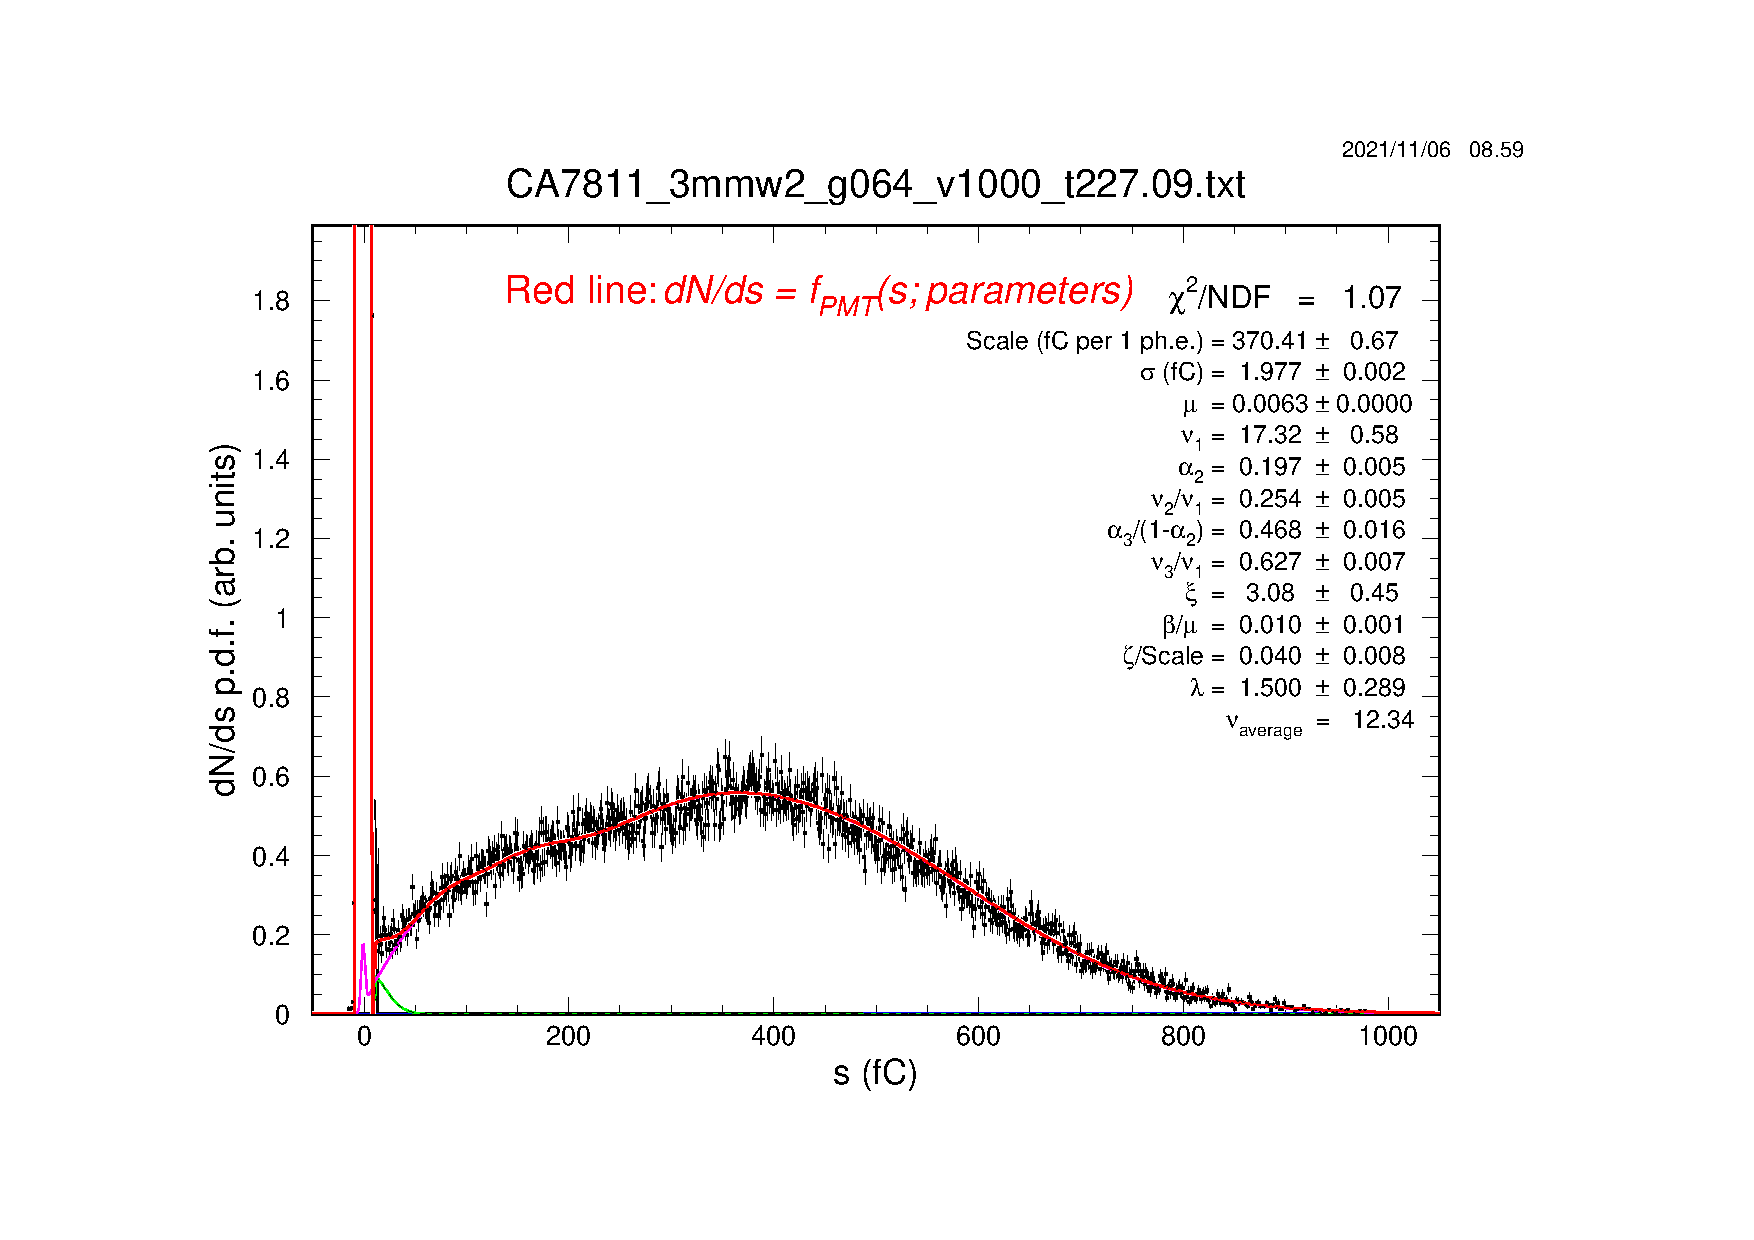
\includegraphics[clip=true,trim=100 75 140 100,width=.245\textwidth,height=.15\textwidth]
                    {figures/CA7811_a.pdf}}
  \subfloat[6 mm mask]{%
    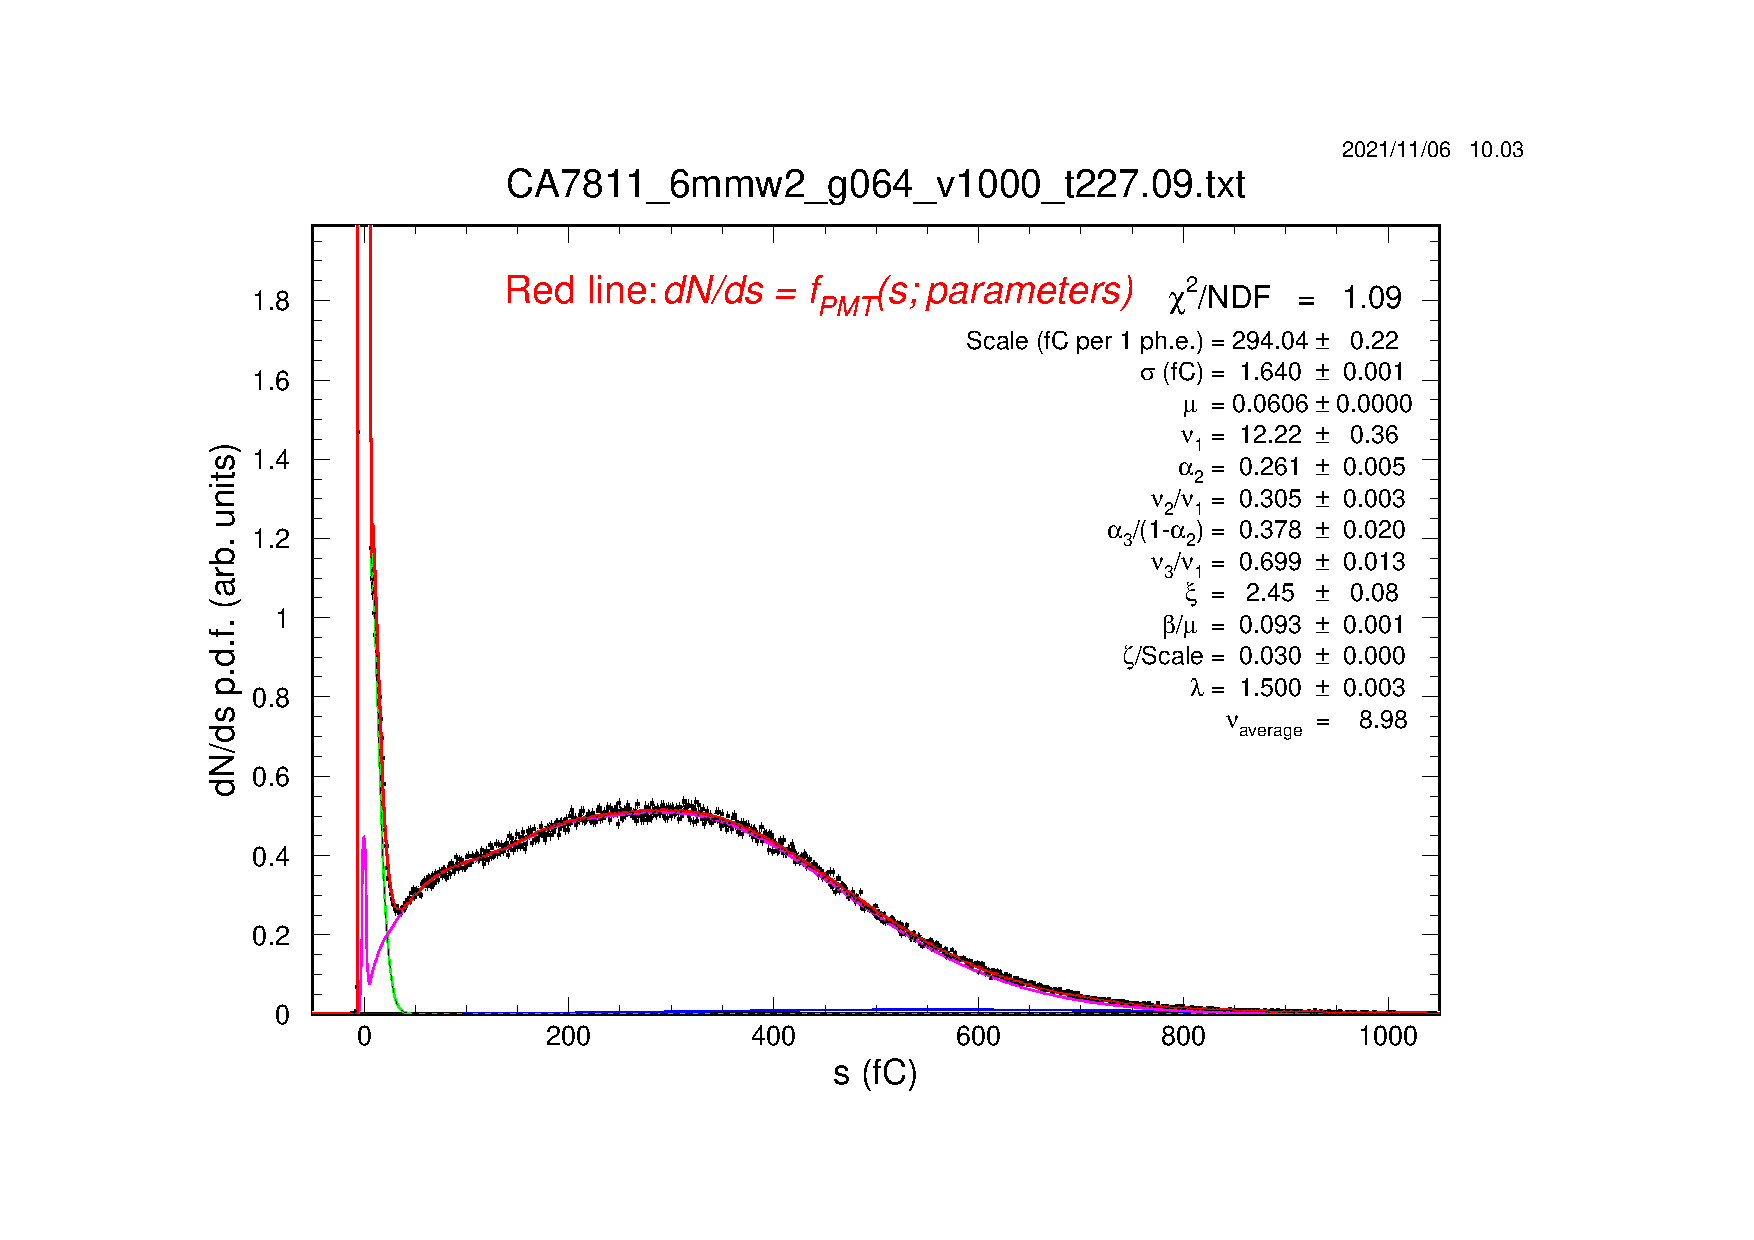
\includegraphics[clip=true,trim=100 75 140 100,width=.245\textwidth,height=.15\textwidth]
                    {figures/CA7811_b.pdf}}
  \subfloat[No mask, cross talk removed by software]{%
    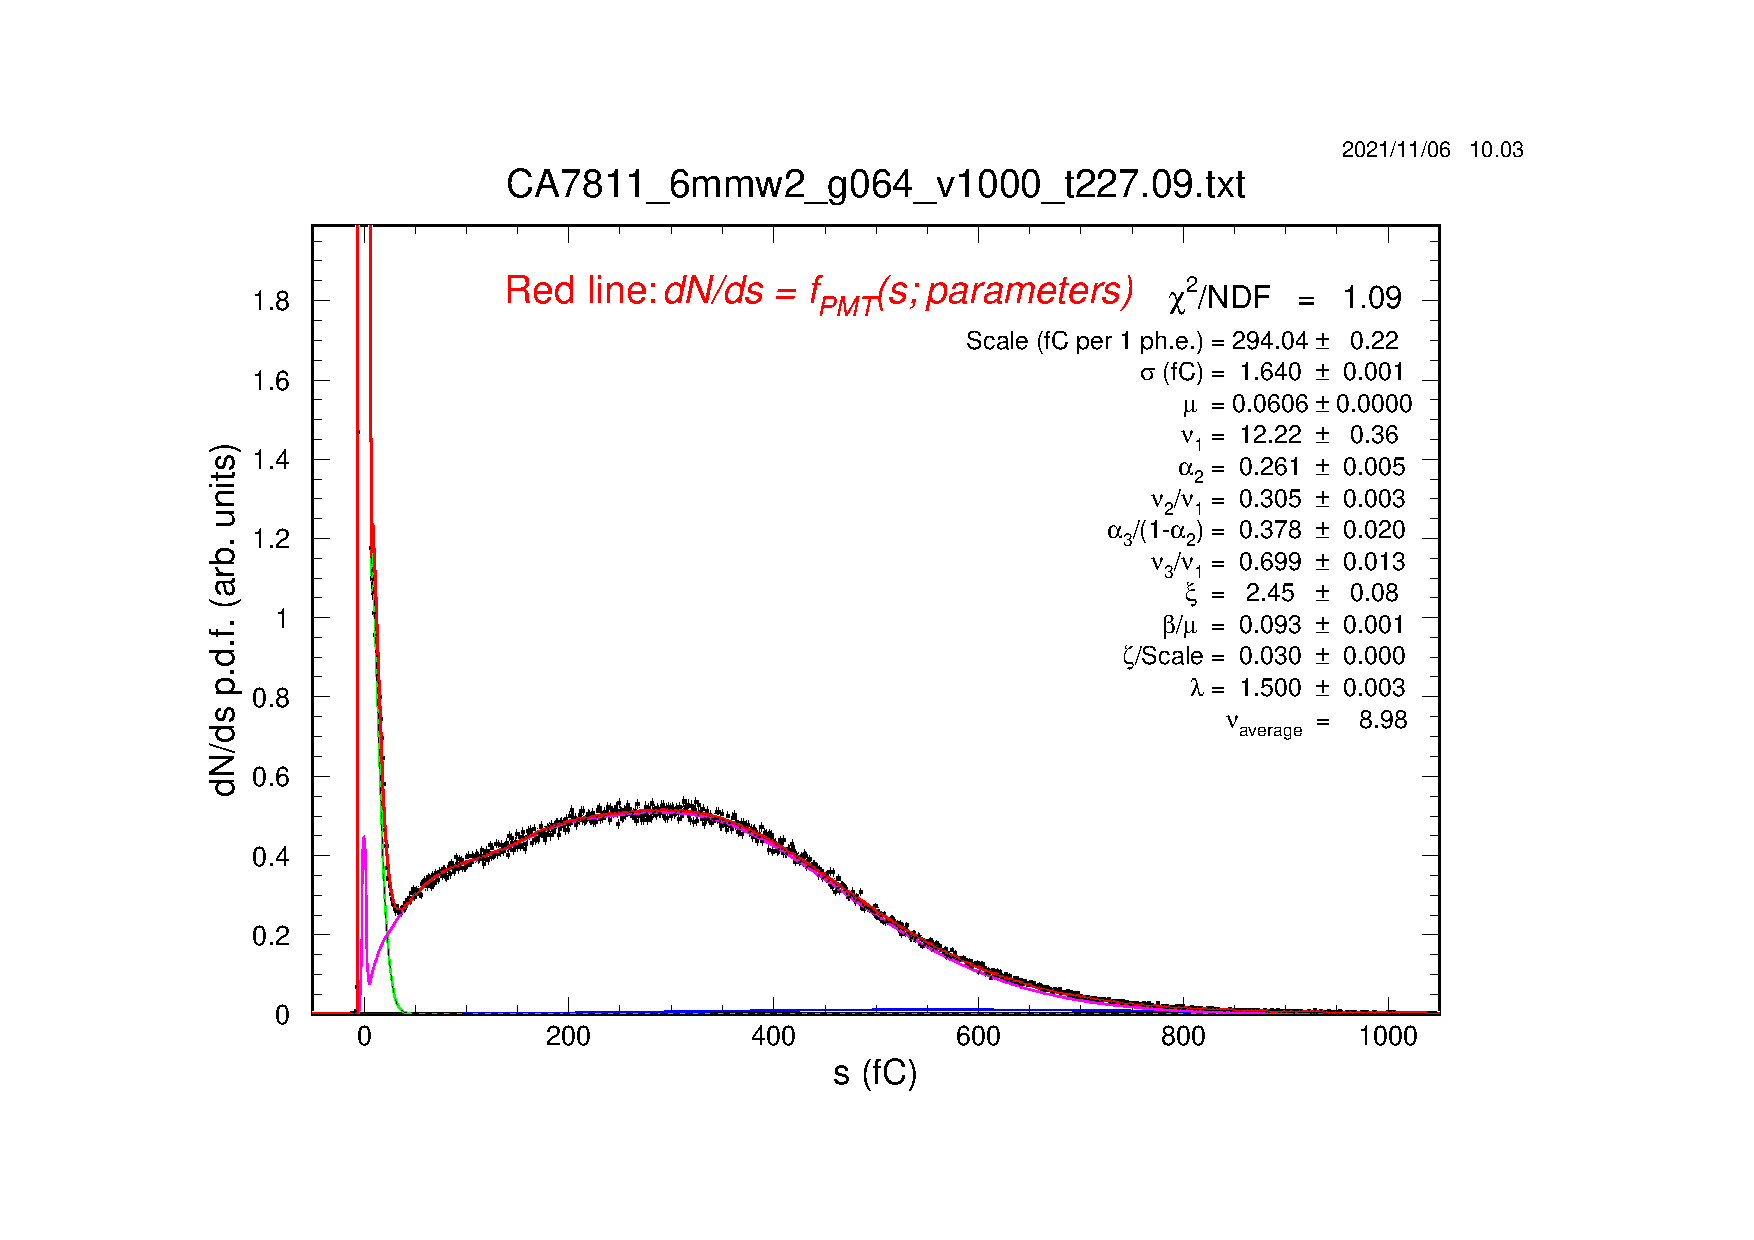
\includegraphics[clip=true,trim=100 75 140 100,width=.245\textwidth,height=.15\textwidth]
                    {figures/CA7811_c.pdf}}
  \subfloat[No mask, cross talk approximated by fit]{%
    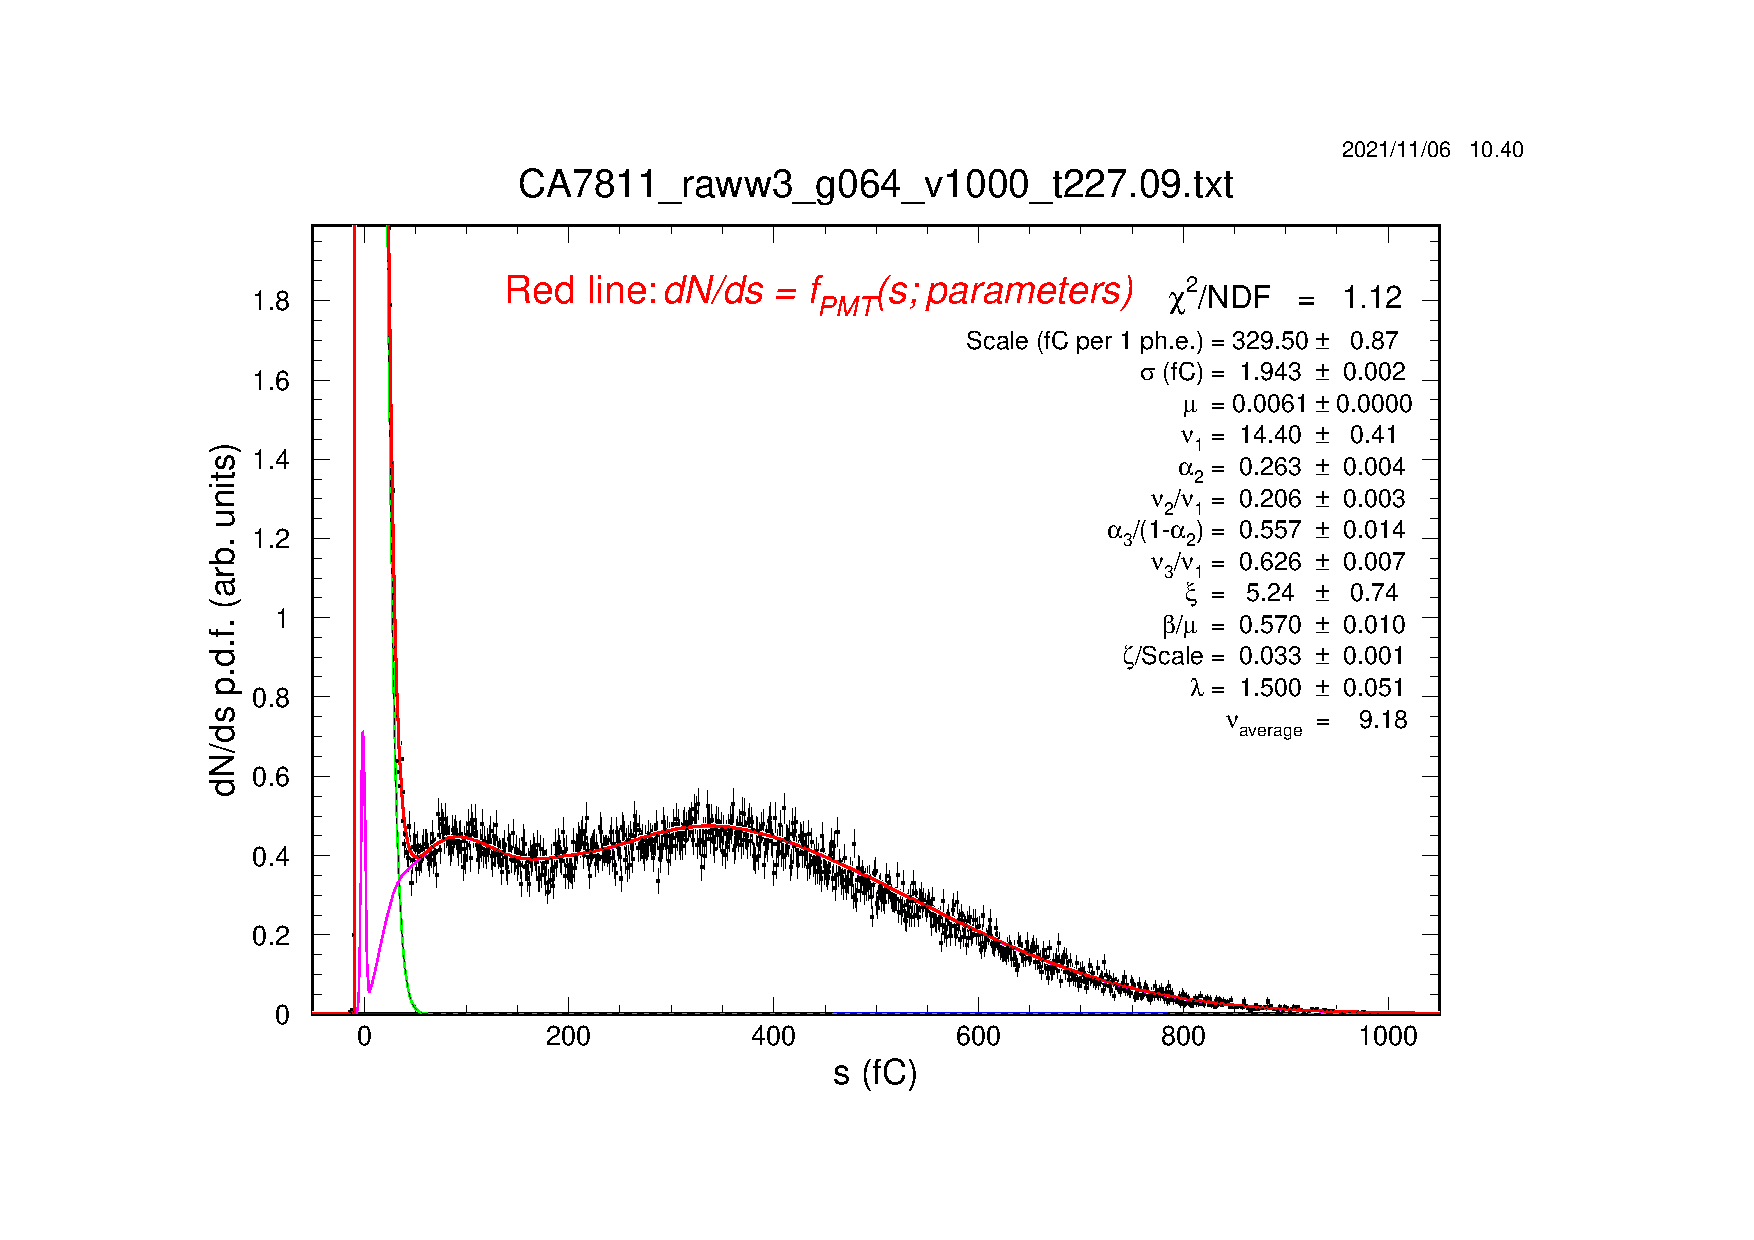
\includegraphics[clip=true,trim=100 75 140 100,width=.245\textwidth,height=.15\textwidth]
                    {figures/CA7811_d.pdf}}
  \caption{Signal amplitude probability distributions for PMT CA7811 (H8500), pixel 9, at HV = 1000 V. a) 3mm mask. b) 6mm mask. c) run with full PMT face open, cross-talk events removed by the correlation analysis. d) run with full PMT face open, the contribution to the spectrum from the cross-talk events is approximated and parameterized by the analysis algorithm. The cross talk effects are too wide to be approximated correctly.
    }
\label{fig:CA7811}
\end{figure*}

\begin{figure*}[h!bt] 
\centering 
  \subfloat[3 mm mask]{%
    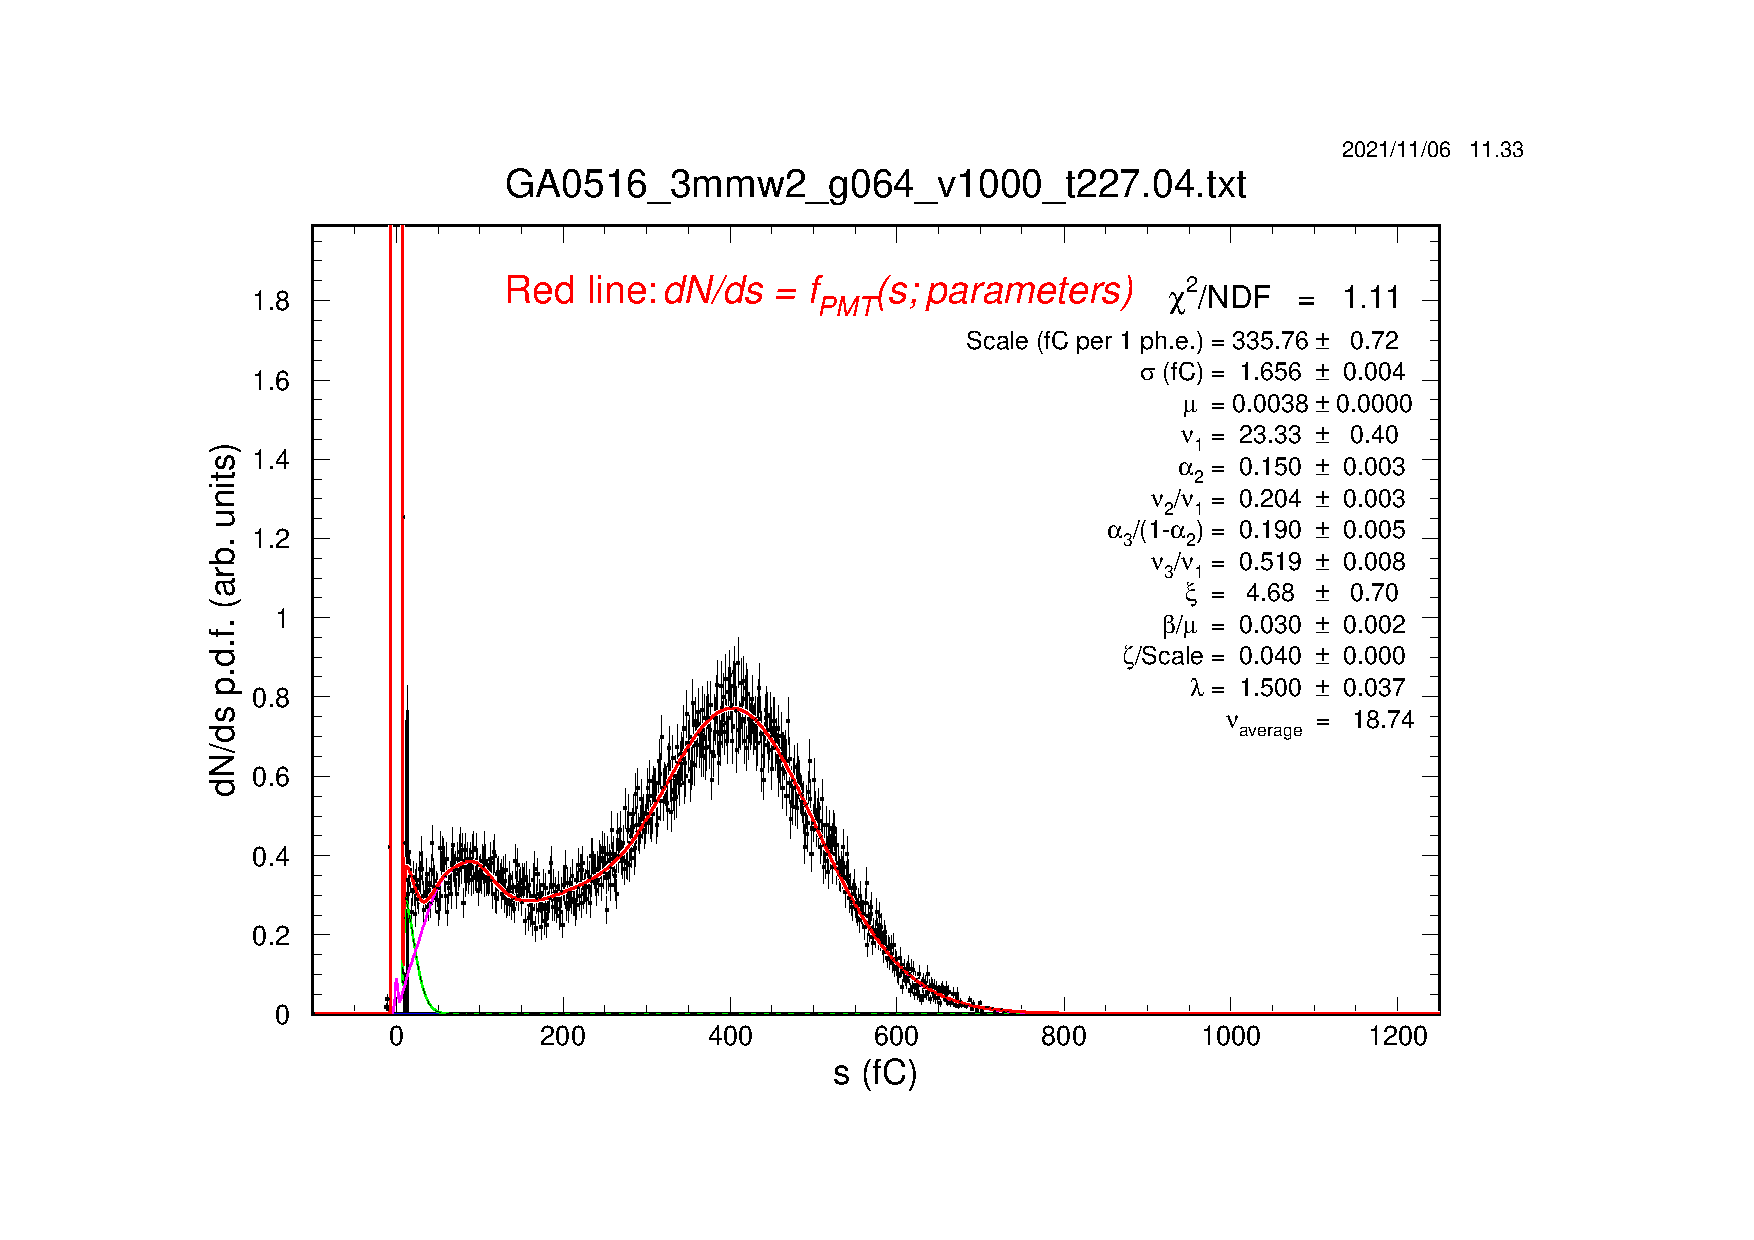
\includegraphics[clip=true,trim=100 75 140 100,width=.245\textwidth,height=.15\textwidth]
                    {figures/GA0516_1a.pdf}}
  \subfloat[6 mm mask]{%
    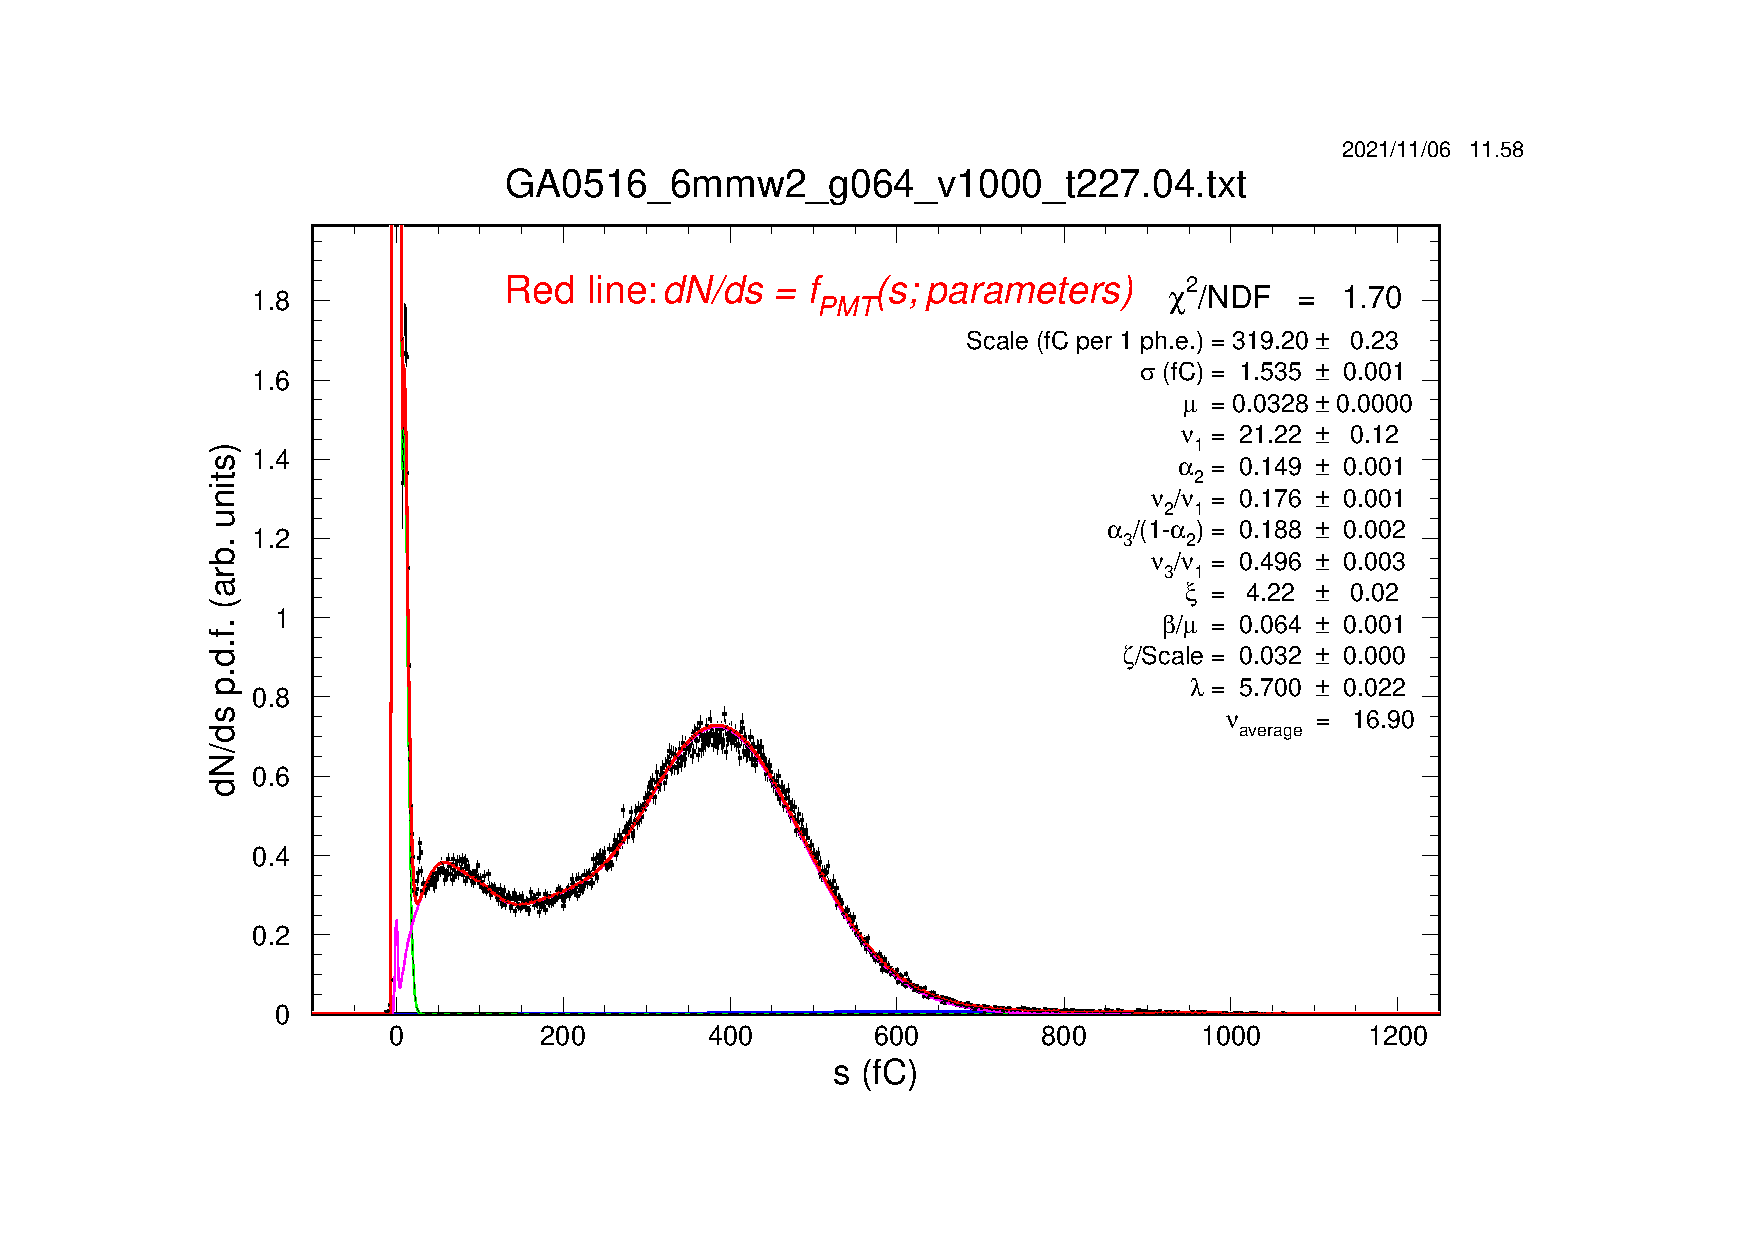
\includegraphics[clip=true,trim=100 75 140 100,width=.245\textwidth,height=.15\textwidth]
                    {figures/GA0516_1b.pdf}}
  \subfloat[No mask, cross talk removed by software]{%
    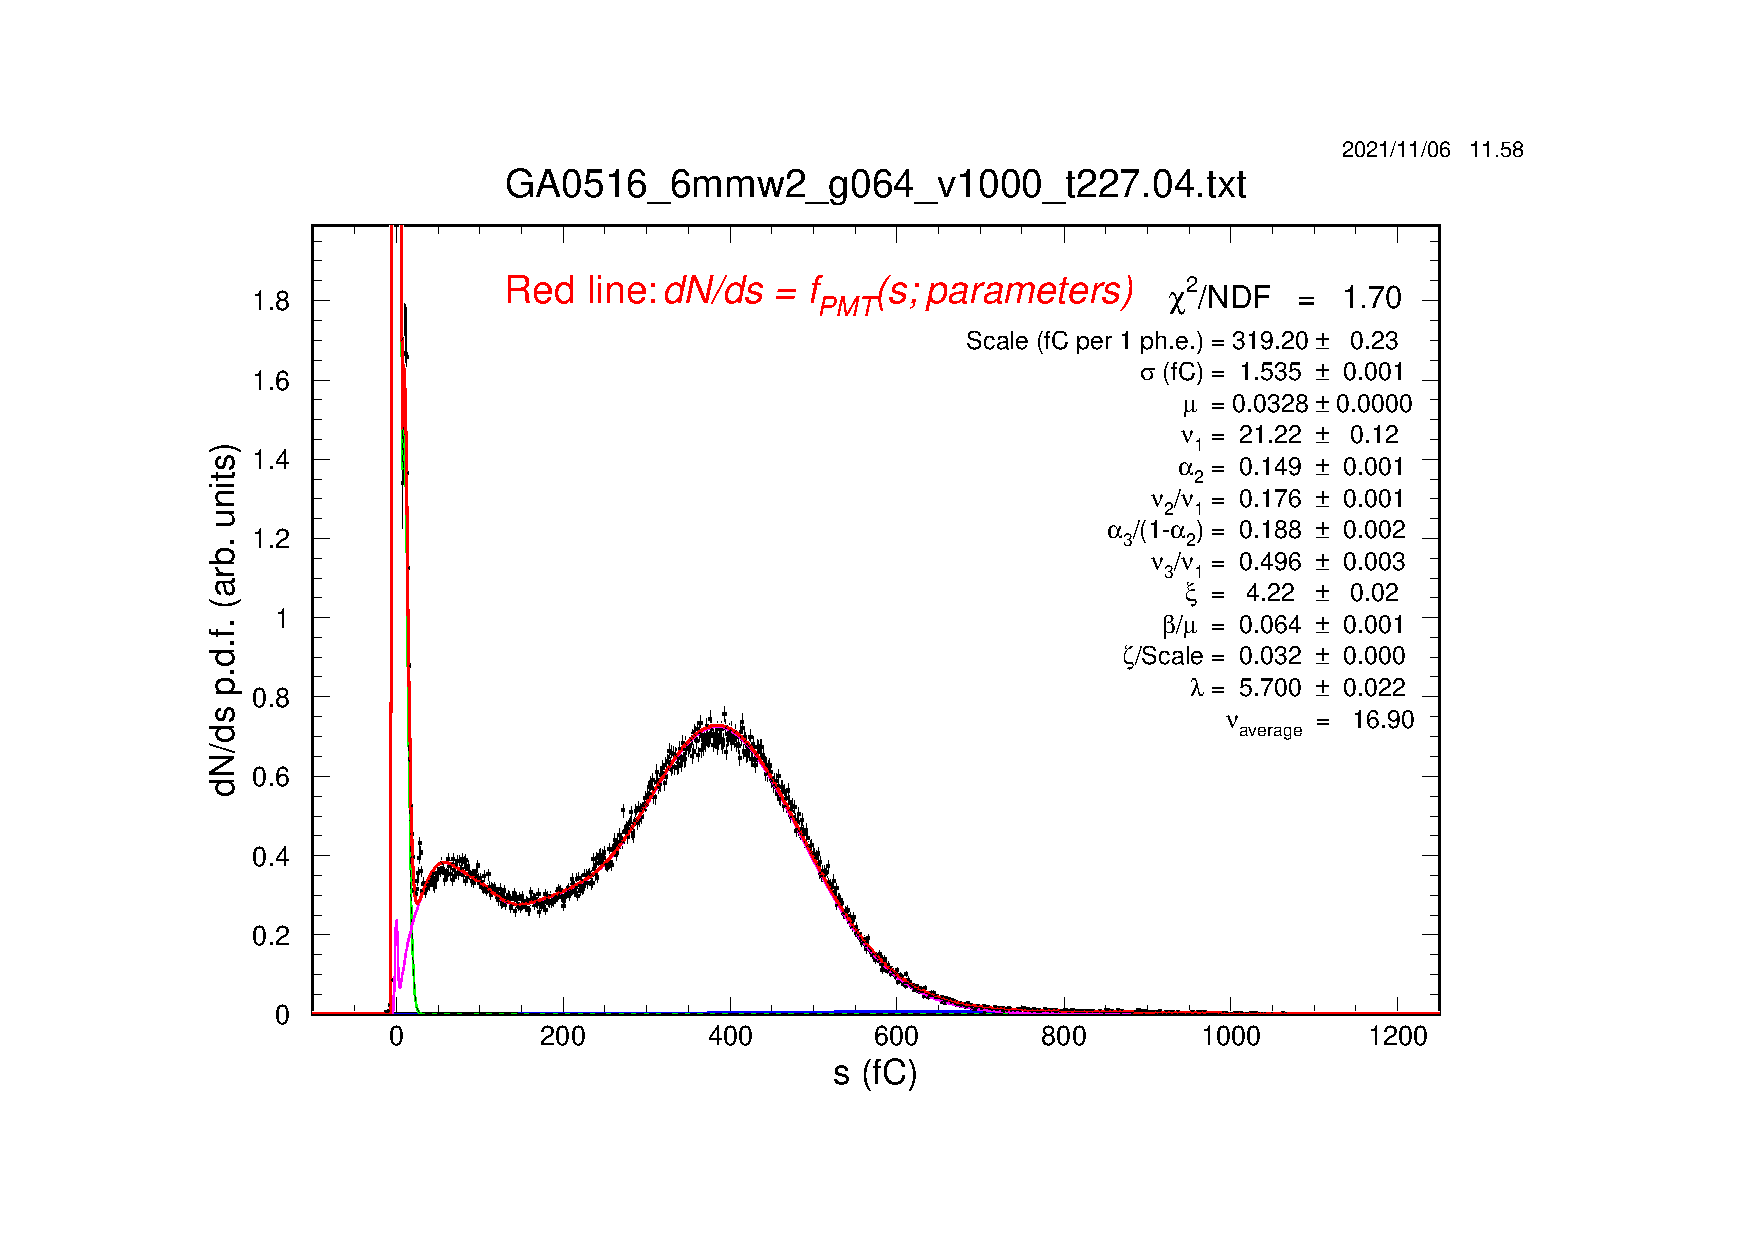
\includegraphics[clip=true,trim=100 75 140 100,width=.245\textwidth,height=.15\textwidth]
                    {figures/GA0516_1c.pdf}}
  \subfloat[No mask, cross talk approximated by fit]{%
    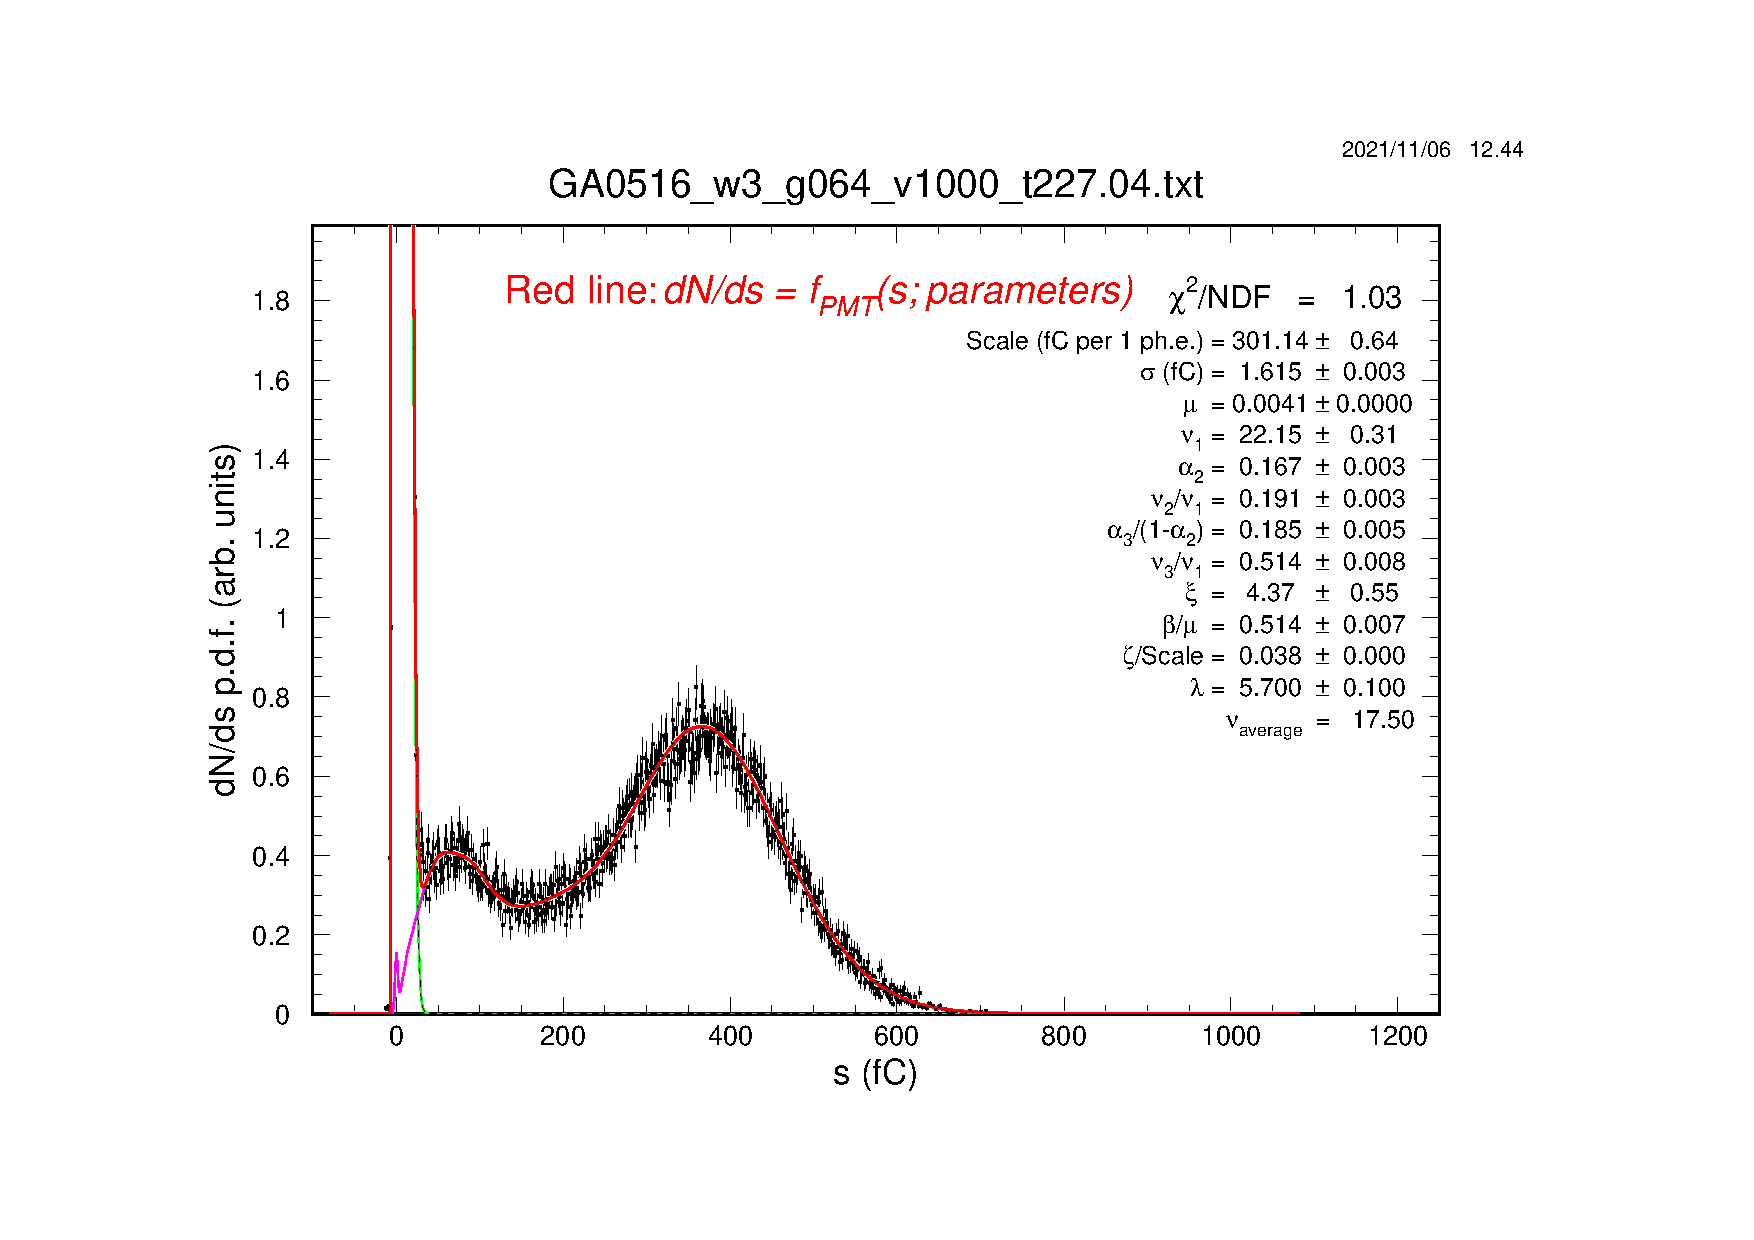
\includegraphics[clip=true,trim=100 75 140 100,width=.245\textwidth,height=.15\textwidth]
                    {figures/GA0516_1d.pdf}}
  \caption{Signal amplitude probability distributions for PMT GA0516 (H12700), pixel 4, at HV = 1000 V. a) 3mm mask. b) 6mm mask. c) run with full PMT face open, cross-talk events removed by the correlation analysis. d) run with full PMT face open, the contribution to the spectrum from the cross-talk events is approximated and parameterized by the analysis algorithm.
    }
\label{fig:GA0516_1}
\end{figure*}
\begin{figure*}[h!bt] 
\centering 
  \subfloat[3 mm mask]{%
    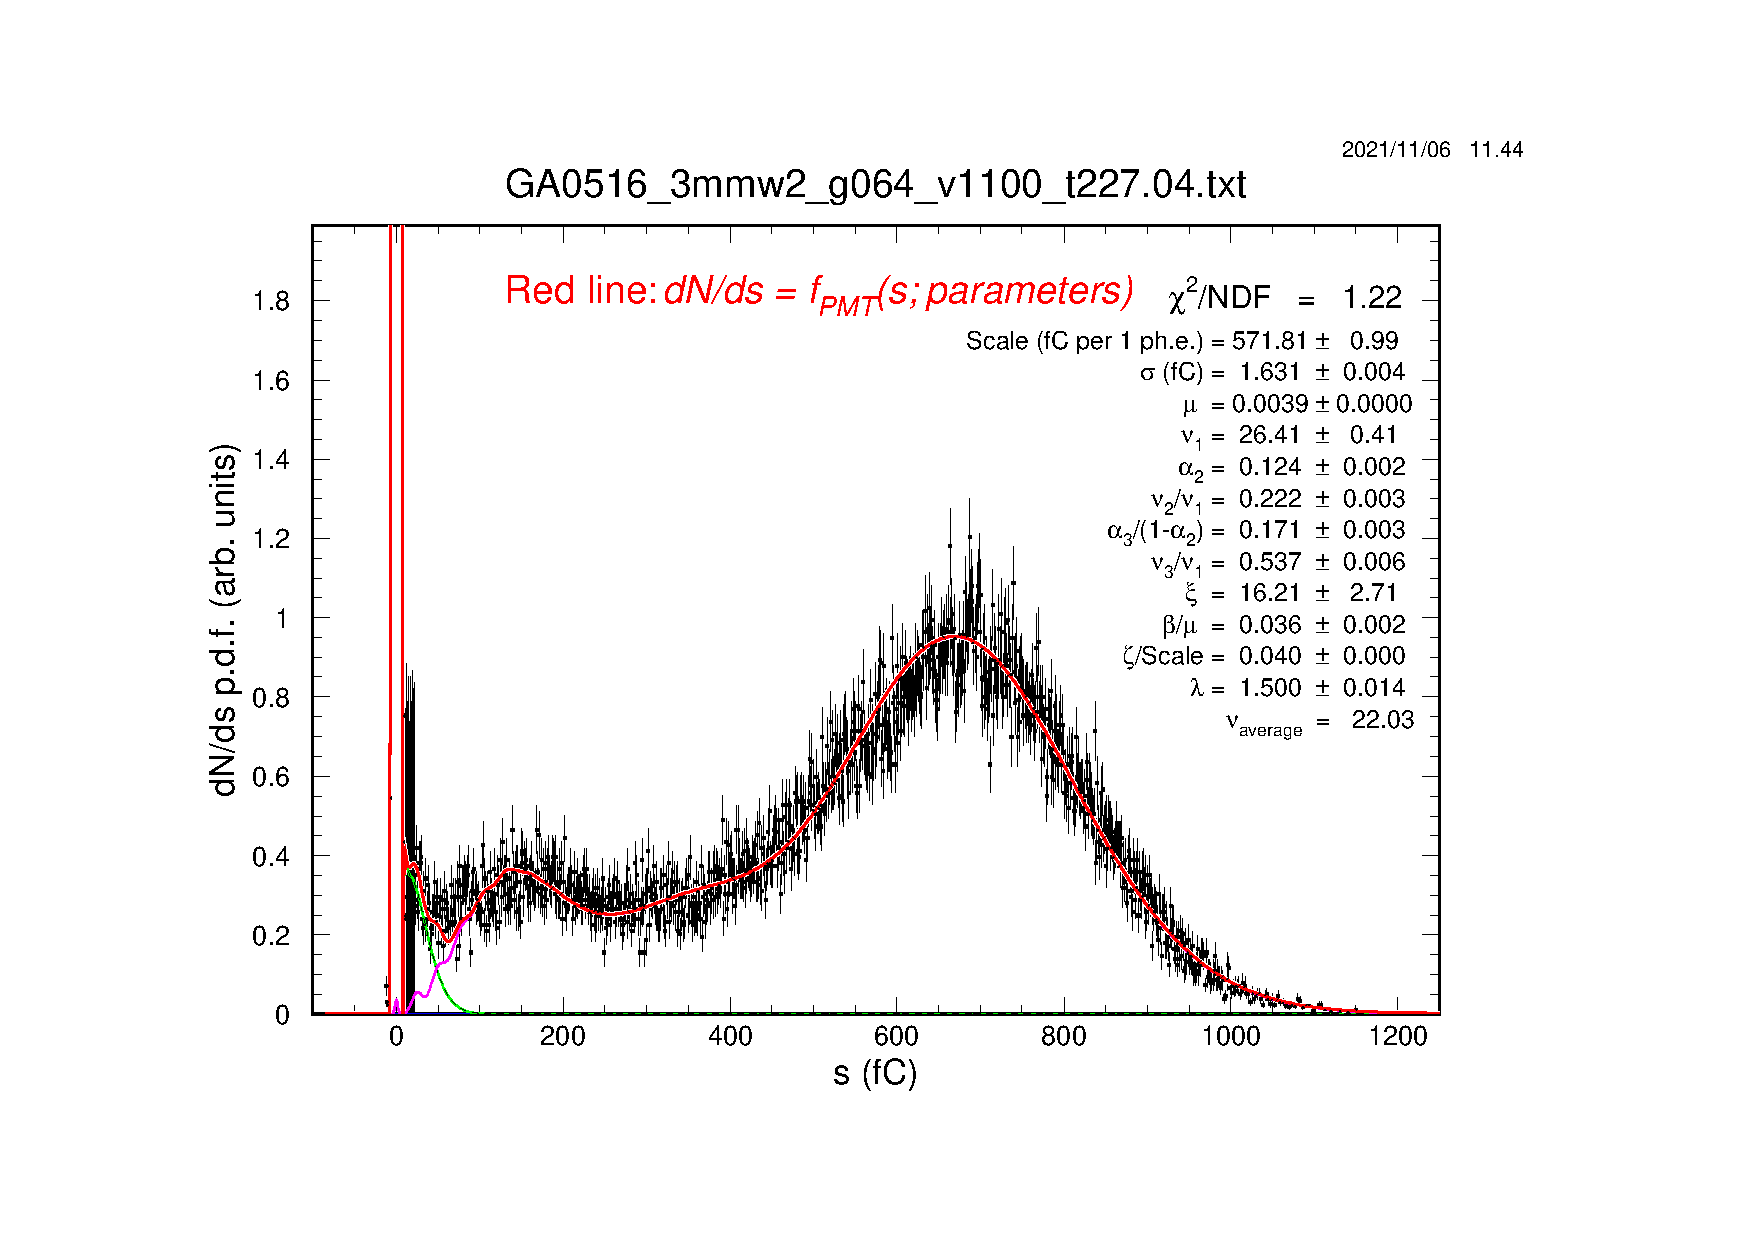
\includegraphics[clip=true,trim=100 75 140 100,width=.245\textwidth,height=.15\textwidth]
                    {figures/GA0516_2a.pdf}}
  \subfloat[6 mm mask]{%
    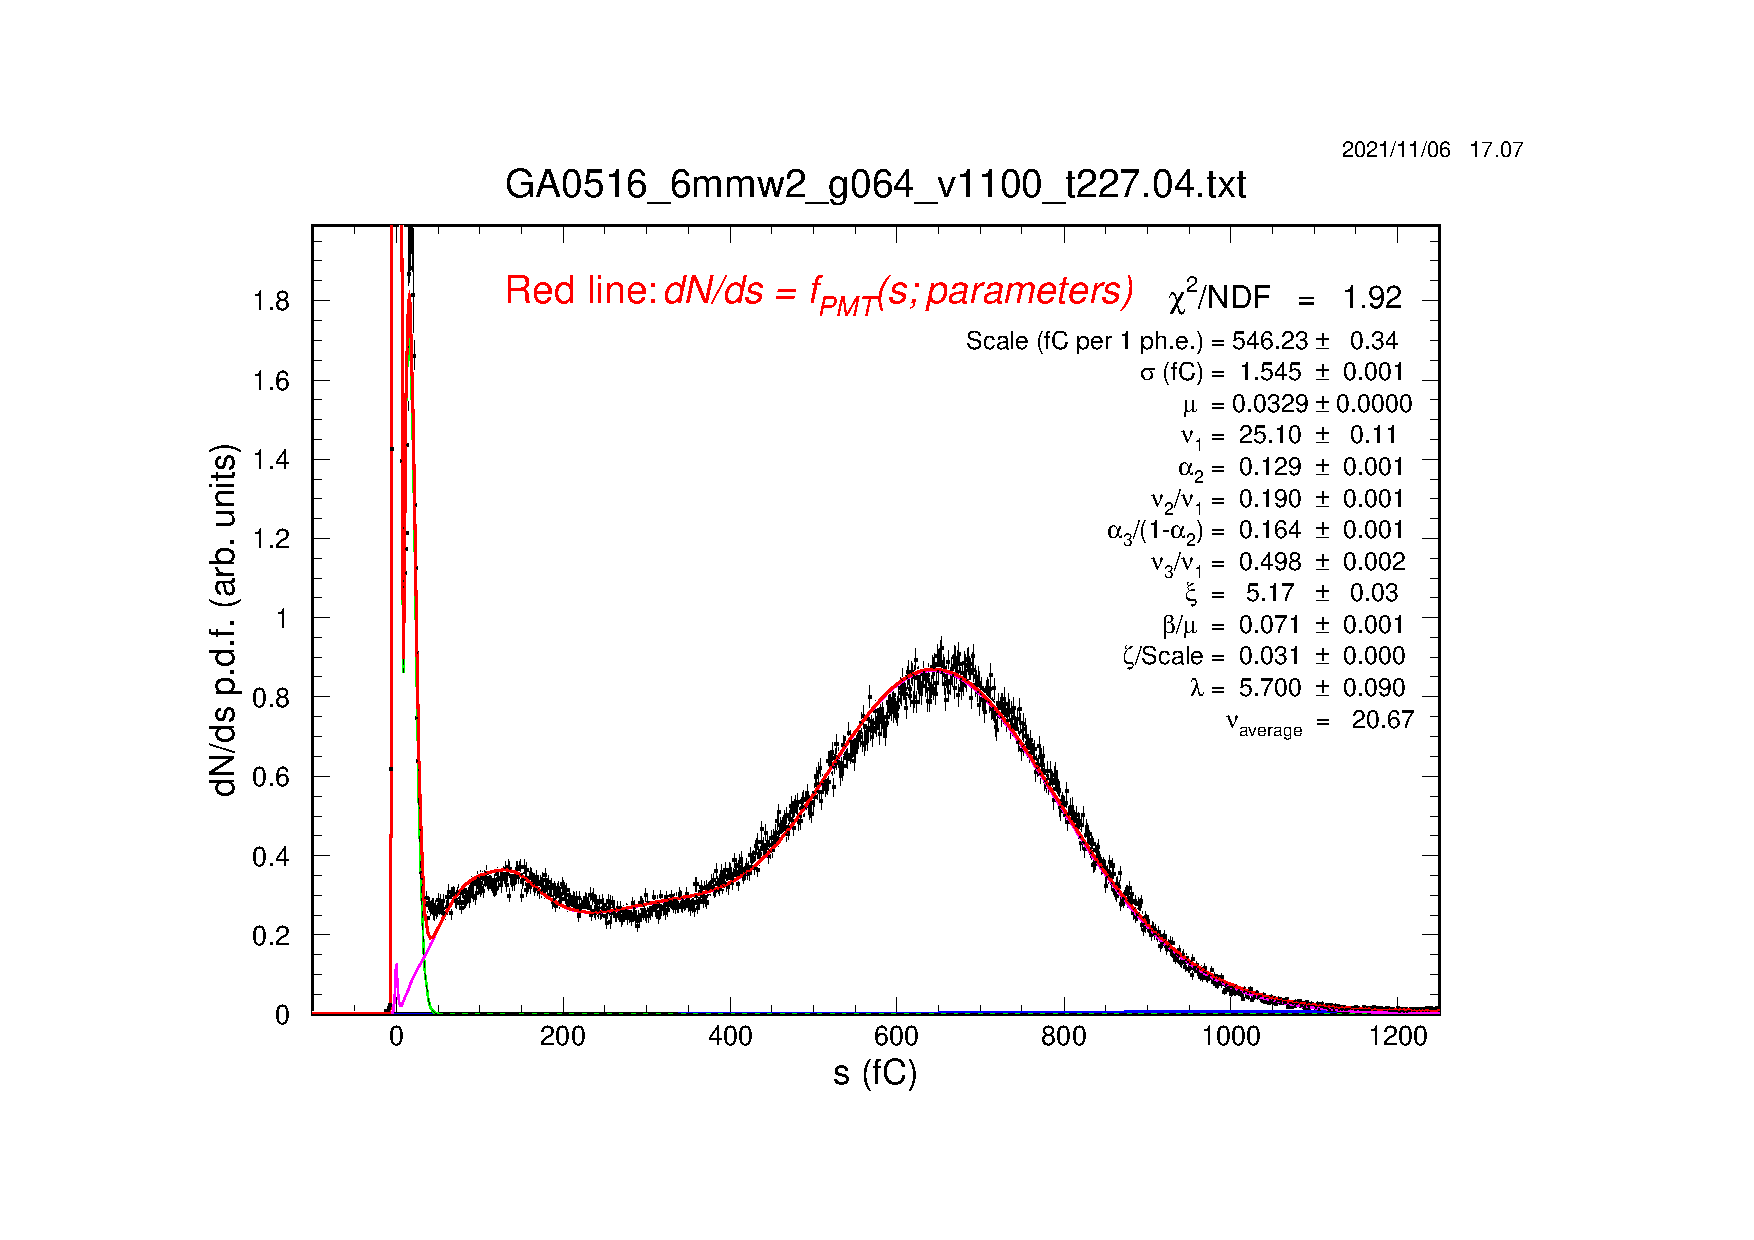
\includegraphics[clip=true,trim=100 75 140 100,width=.245\textwidth,height=.15\textwidth]
                    {figures/GA0516_2b.pdf}}
  \subfloat[No mask, cross talk removed by software]{%
    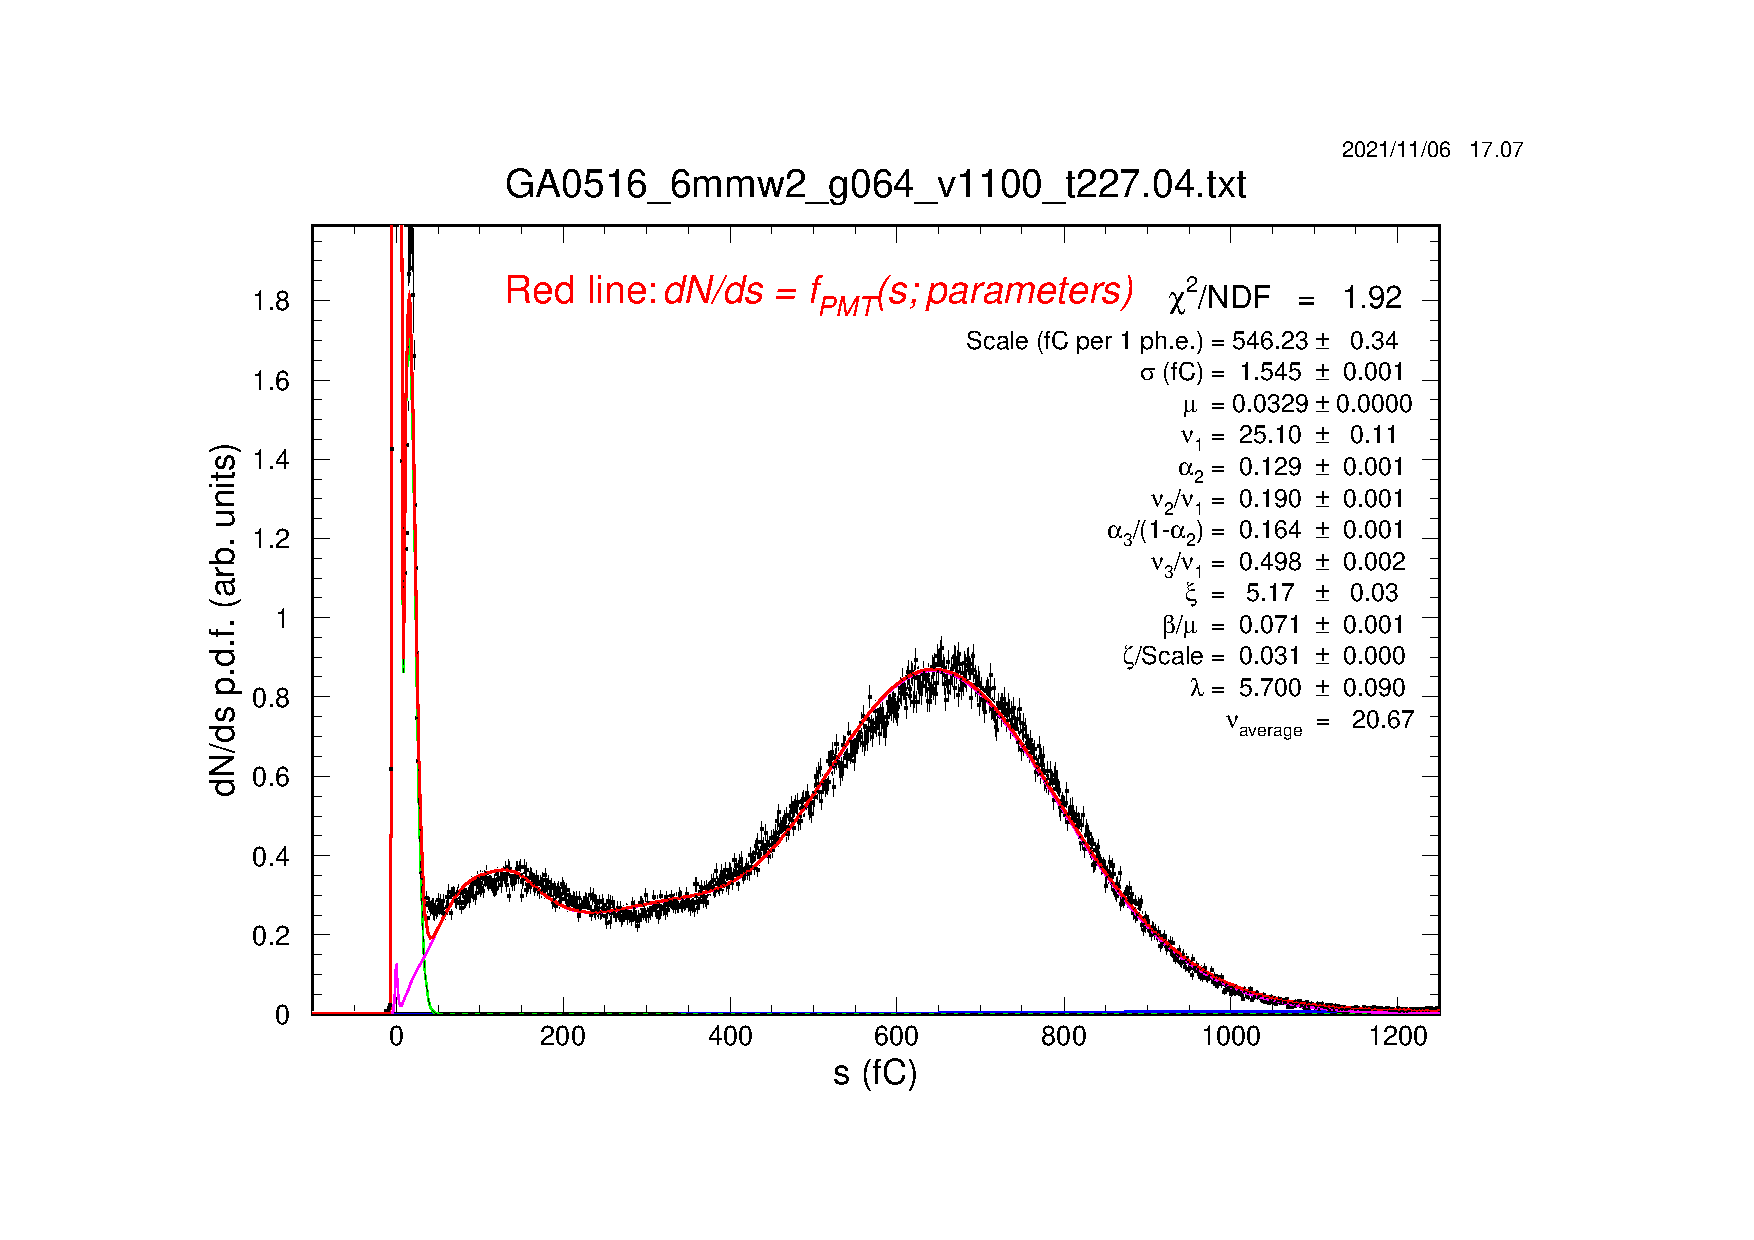
\includegraphics[clip=true,trim=100 75 140 100,width=.245\textwidth,height=.15\textwidth]
                    {figures/GA0516_2c.pdf}}
  \subfloat[No mask, cross talk approximated by fit]{%
    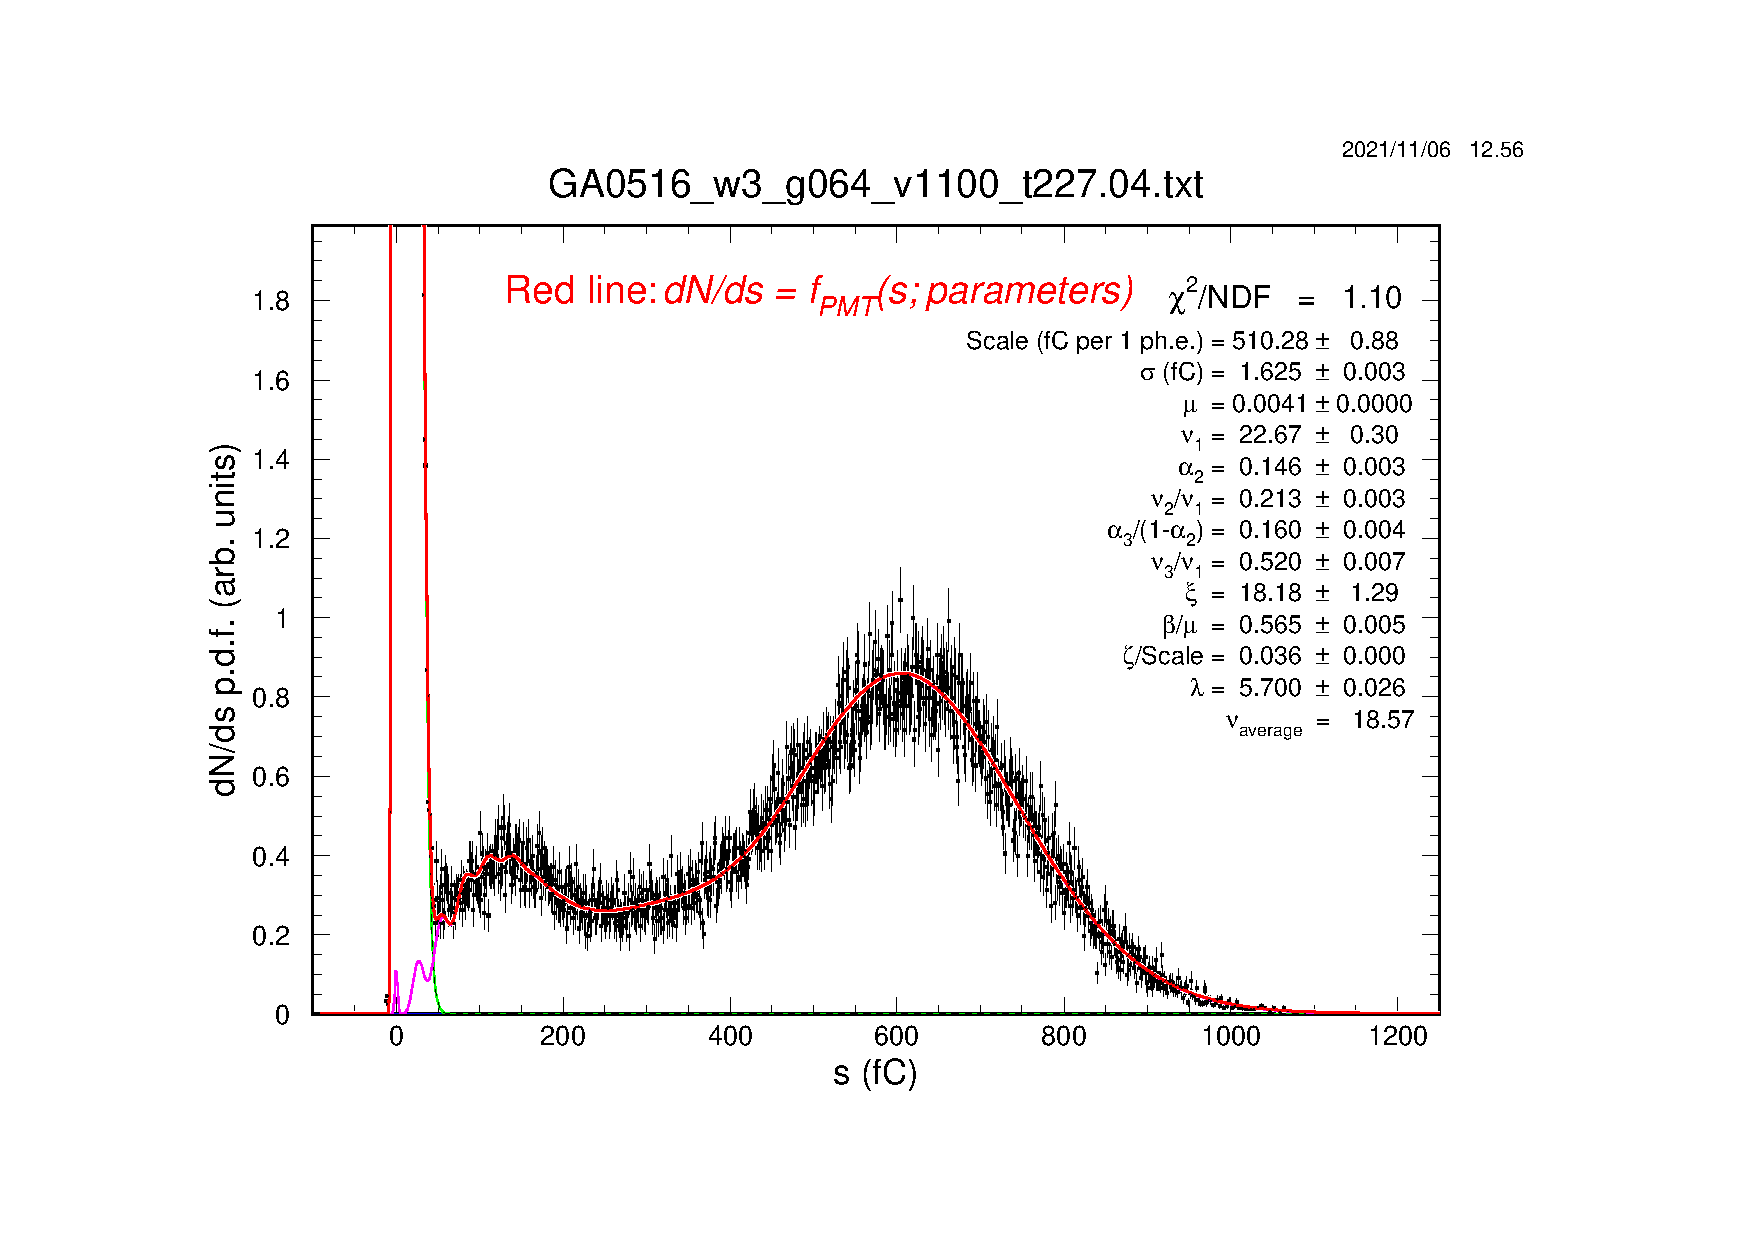
\includegraphics[clip=true,trim=100 75 140 100,width=.245\textwidth,height=.15\textwidth]
                    {figures/GA0516_2d.pdf}}
  \caption{Same as Fig.~\ref{fig:GA0516_1}, but all the data taken at HV = 1100 V. 
    }
\label{fig:GA0516_2}
\end{figure*}
\begin{figure*}[h!bt] 
\centering 
  \subfloat[6 mm mask, at HV = 1000 V]{%
    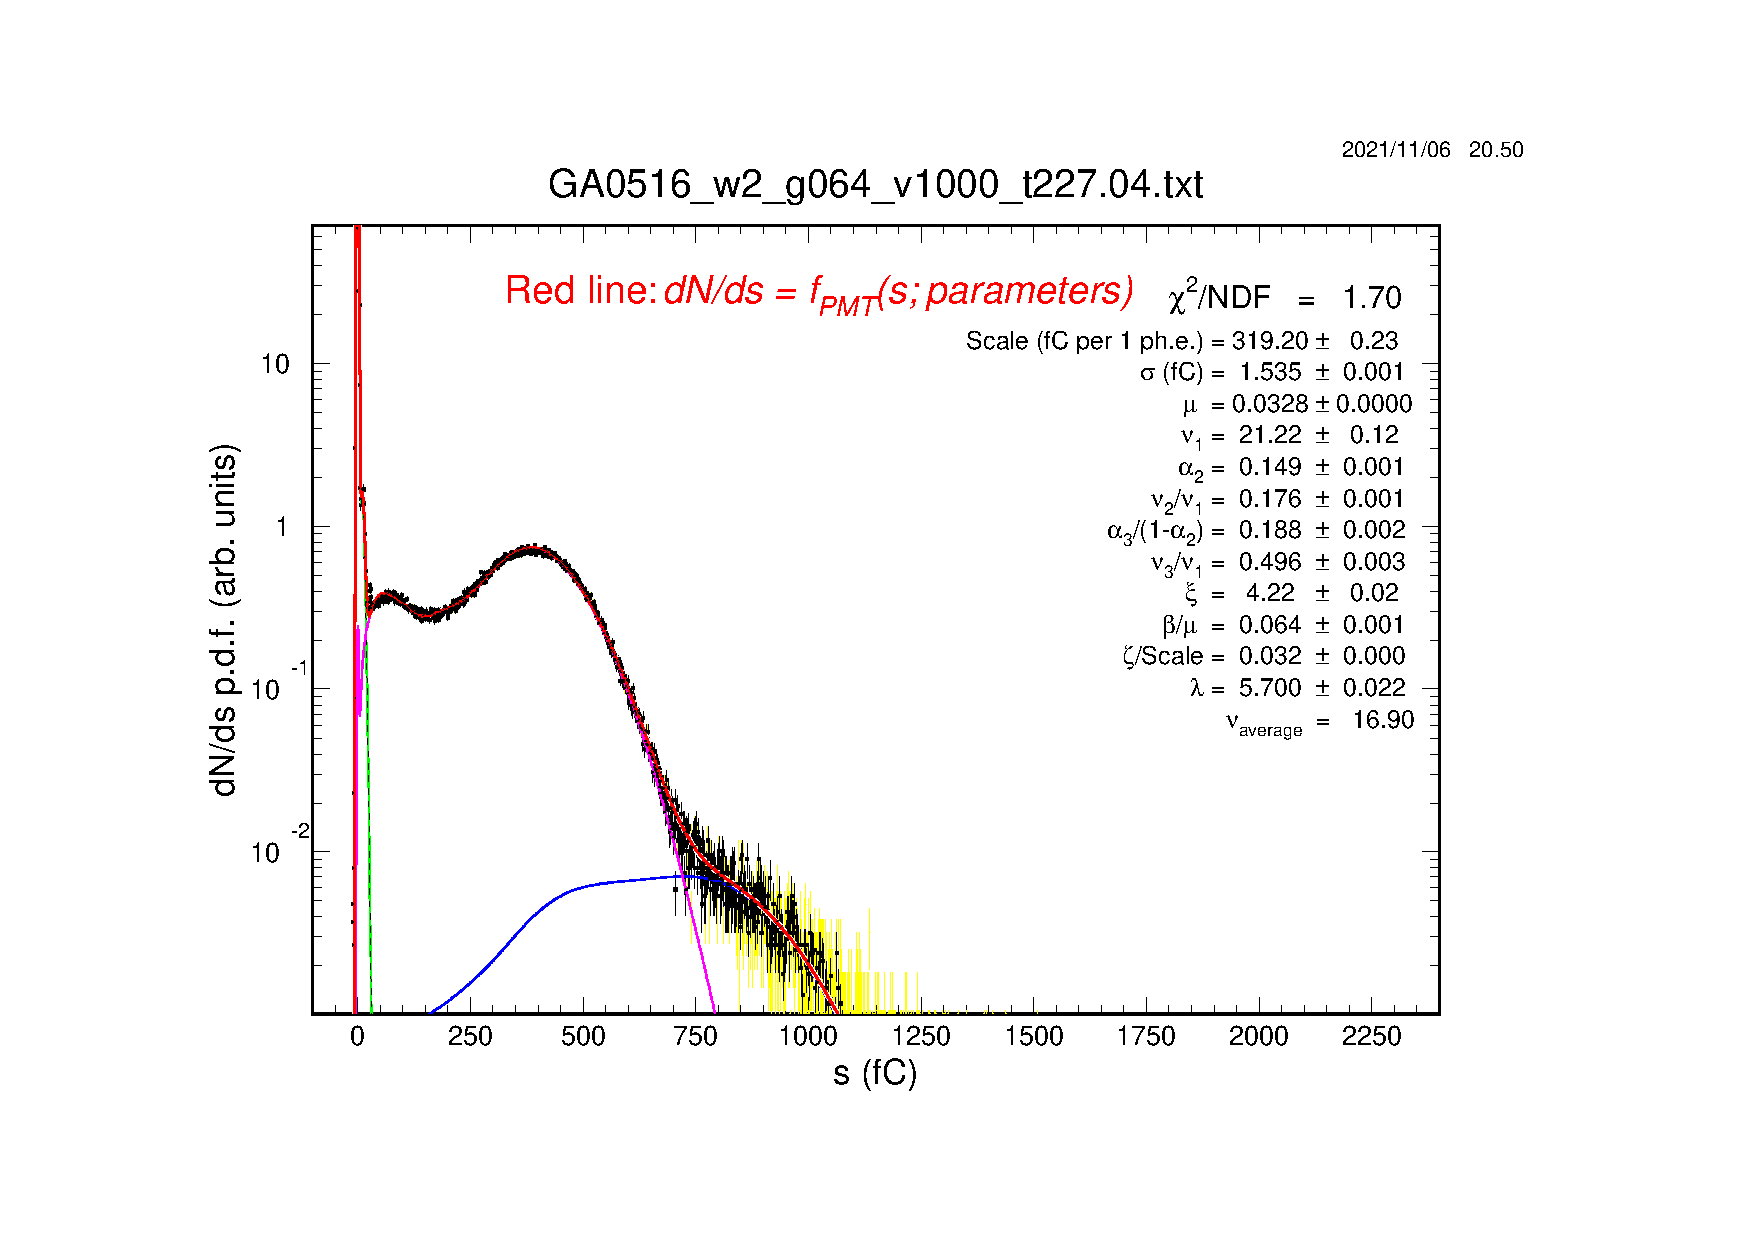
\includegraphics[clip=true,trim=100 75 140 100,width=.245\textwidth,height=.15\textwidth]
                    {figures/GA0516_3a.pdf}}
  \subfloat[6 mm mask, at HV = 1100 V]{%
    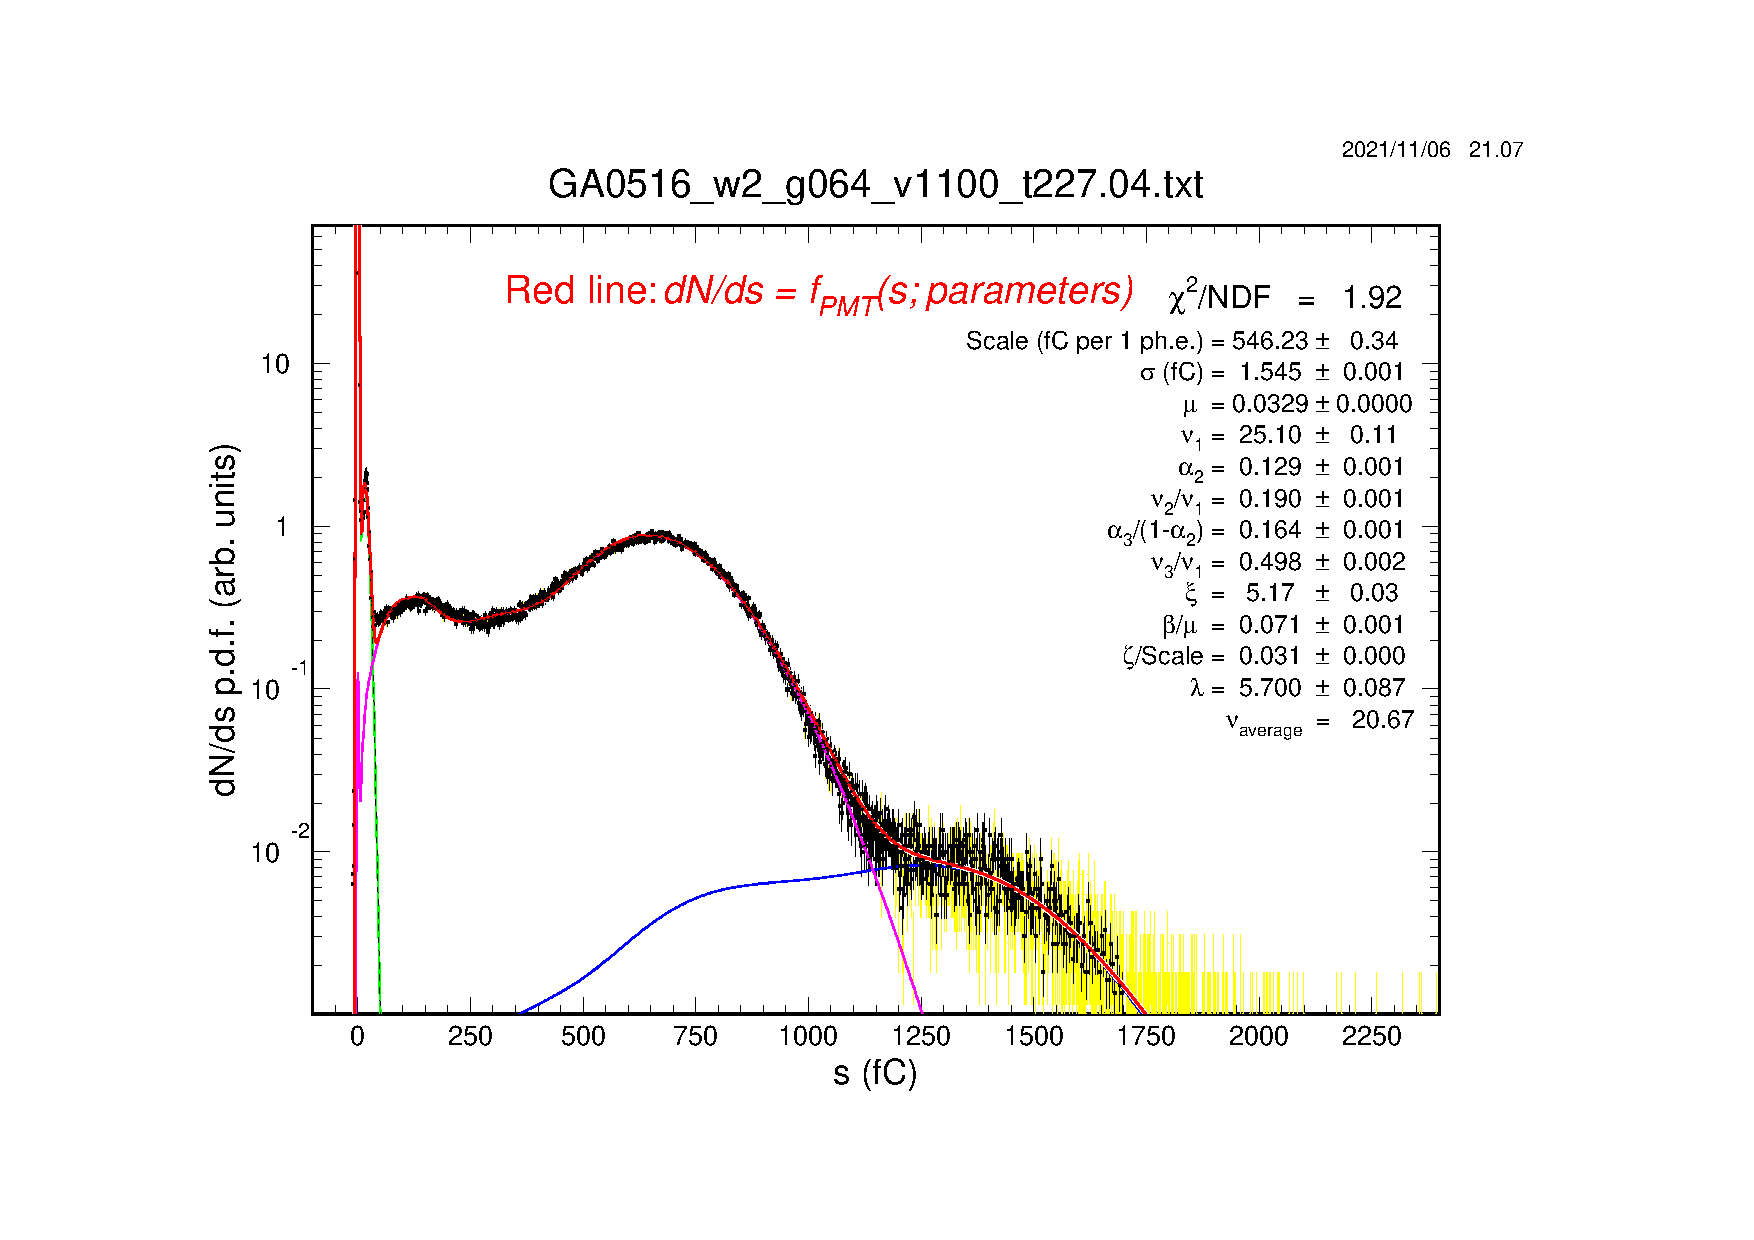
\includegraphics[clip=true,trim=100 75 140 100,width=.245\textwidth,height=.15\textwidth]
                    {figures/GA0516_3b.pdf}}
  \subfloat[No mask, at HV = 1000 V]{%
    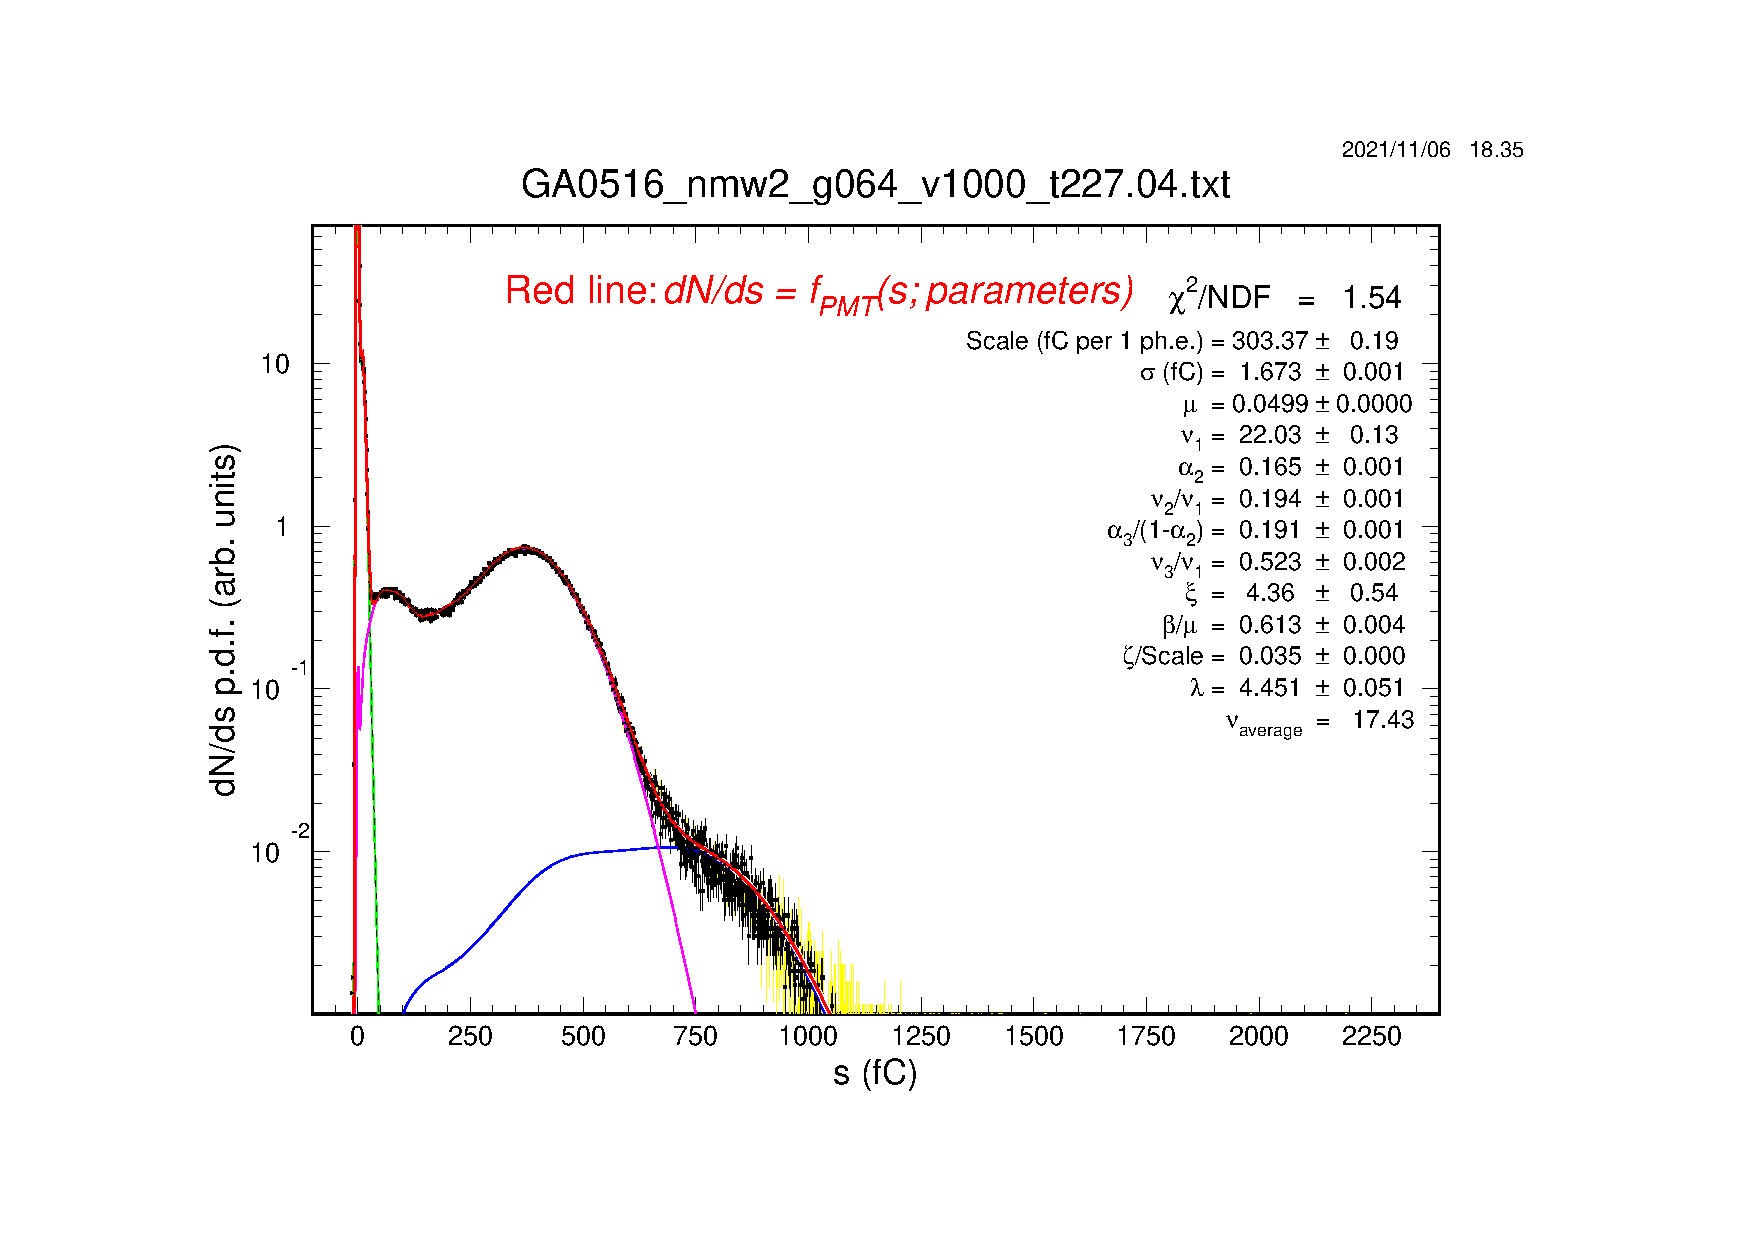
\includegraphics[clip=true,trim=100 75 140 100,width=.245\textwidth,height=.15\textwidth]
                    {figures/GA0516_3c.pdf}}
  \subfloat[No mask, at HV = 1100 V]{%
    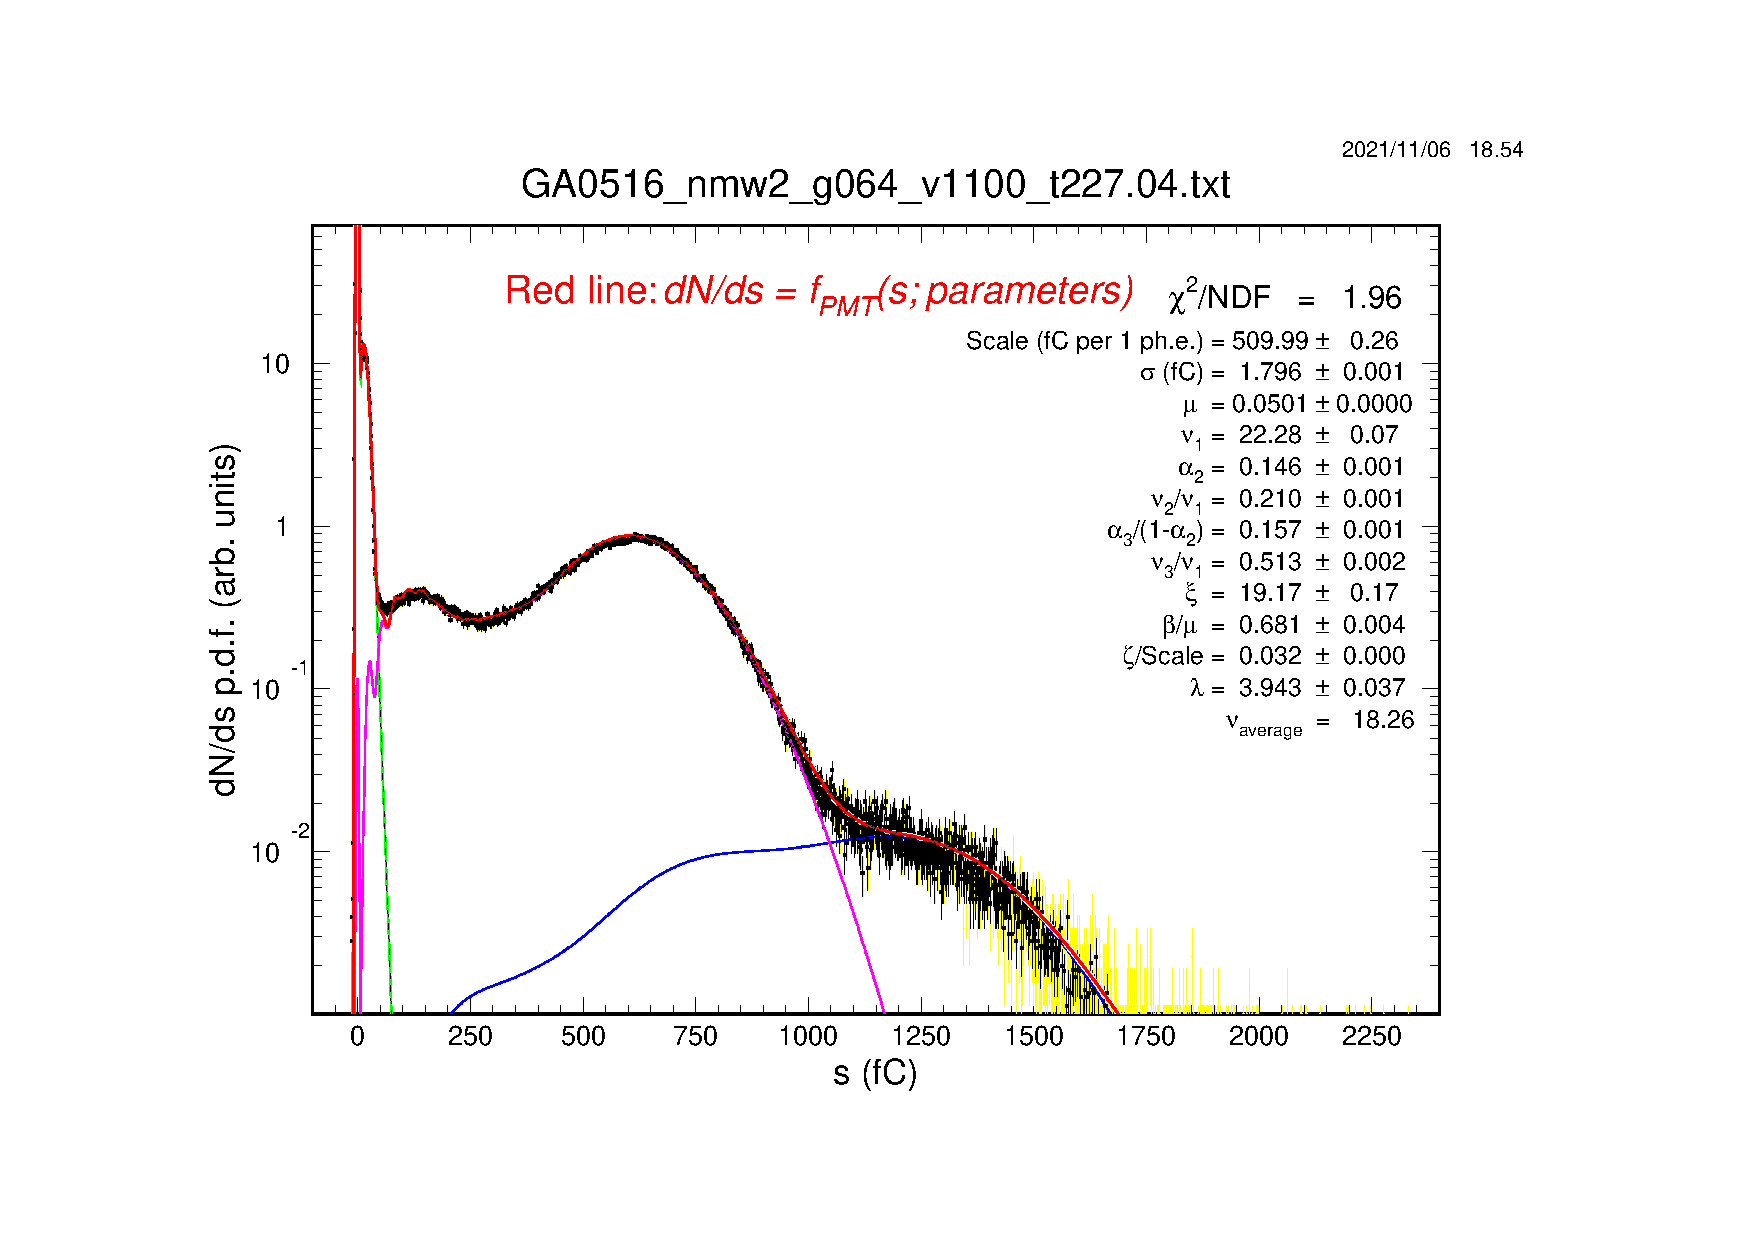
\includegraphics[clip=true,trim=100 75 140 100,width=.245\textwidth,height=.15\textwidth]
                    {figures/GA0516_3d.pdf}}
  \caption{Signal amplitude probability distributions for PMT GA0516 (H12700), pixel 4, wheel position 2, at HV = 1000 V (left plots) and at HV = 1100 V (right plots). (a) and (b) run with 6 mm mask covering the full PMT face except pixel 4. (c) and (d) run with full PMT face open, the contribution to the spectrum from the crosstalk events is approximated and parametrized by the analysis algorithm. Contributions to the spectra are shown by colors: pink is the single photoelectron, violet - two or more photoelectrons, green-black dashed line shows the measurement function including the pedestal Gaussian and the cross talk contribution. 
    }
\label{fig:GA0516_3}
\end{figure*}
\begin{figure*}[h!bt] 
\centering 
  \subfloat[6 mm mask, at HV = 1000 V]{%
    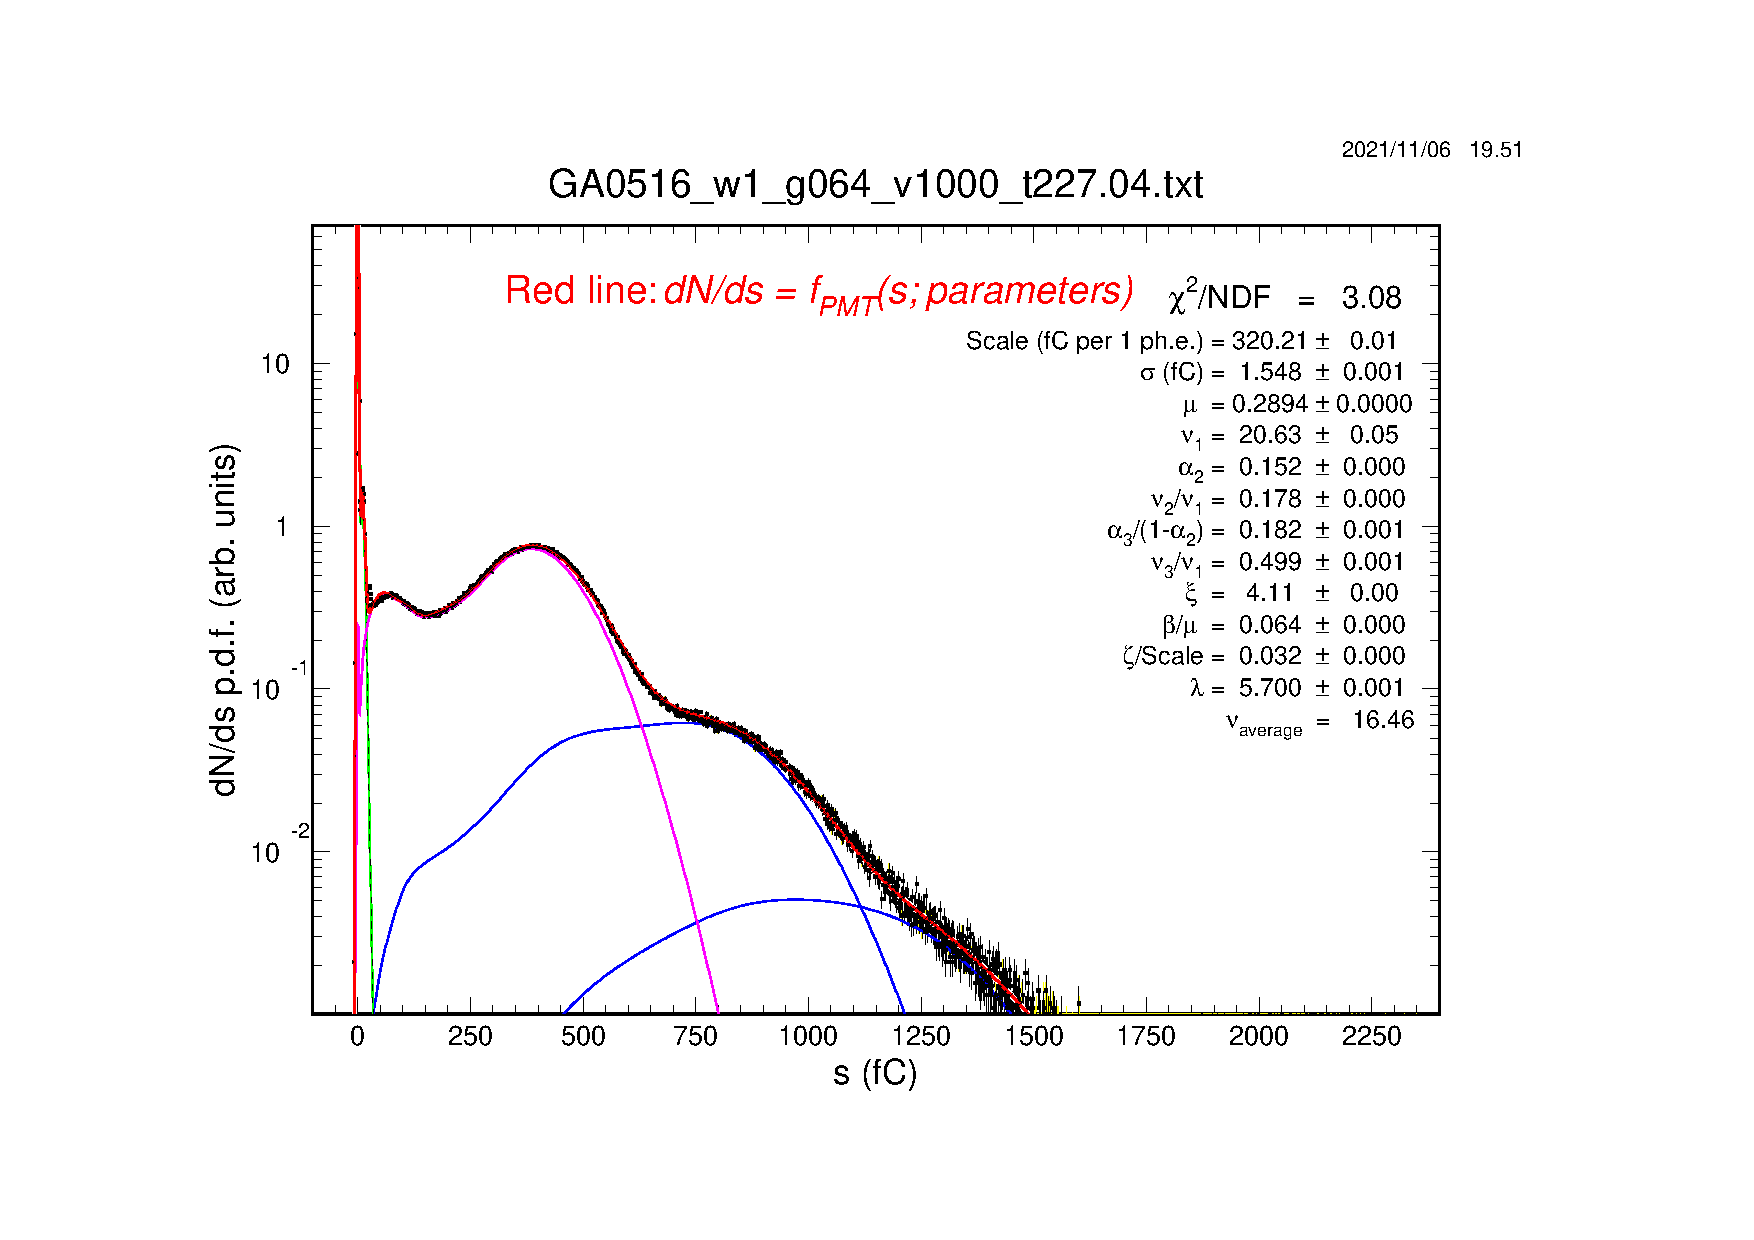
\includegraphics[clip=true,trim=100 75 140 100,width=.245\textwidth,height=.15\textwidth]
                    {figures/GA0516_4a.pdf}}
  \subfloat[6 mm mask, at HV = 1100 V]{%
    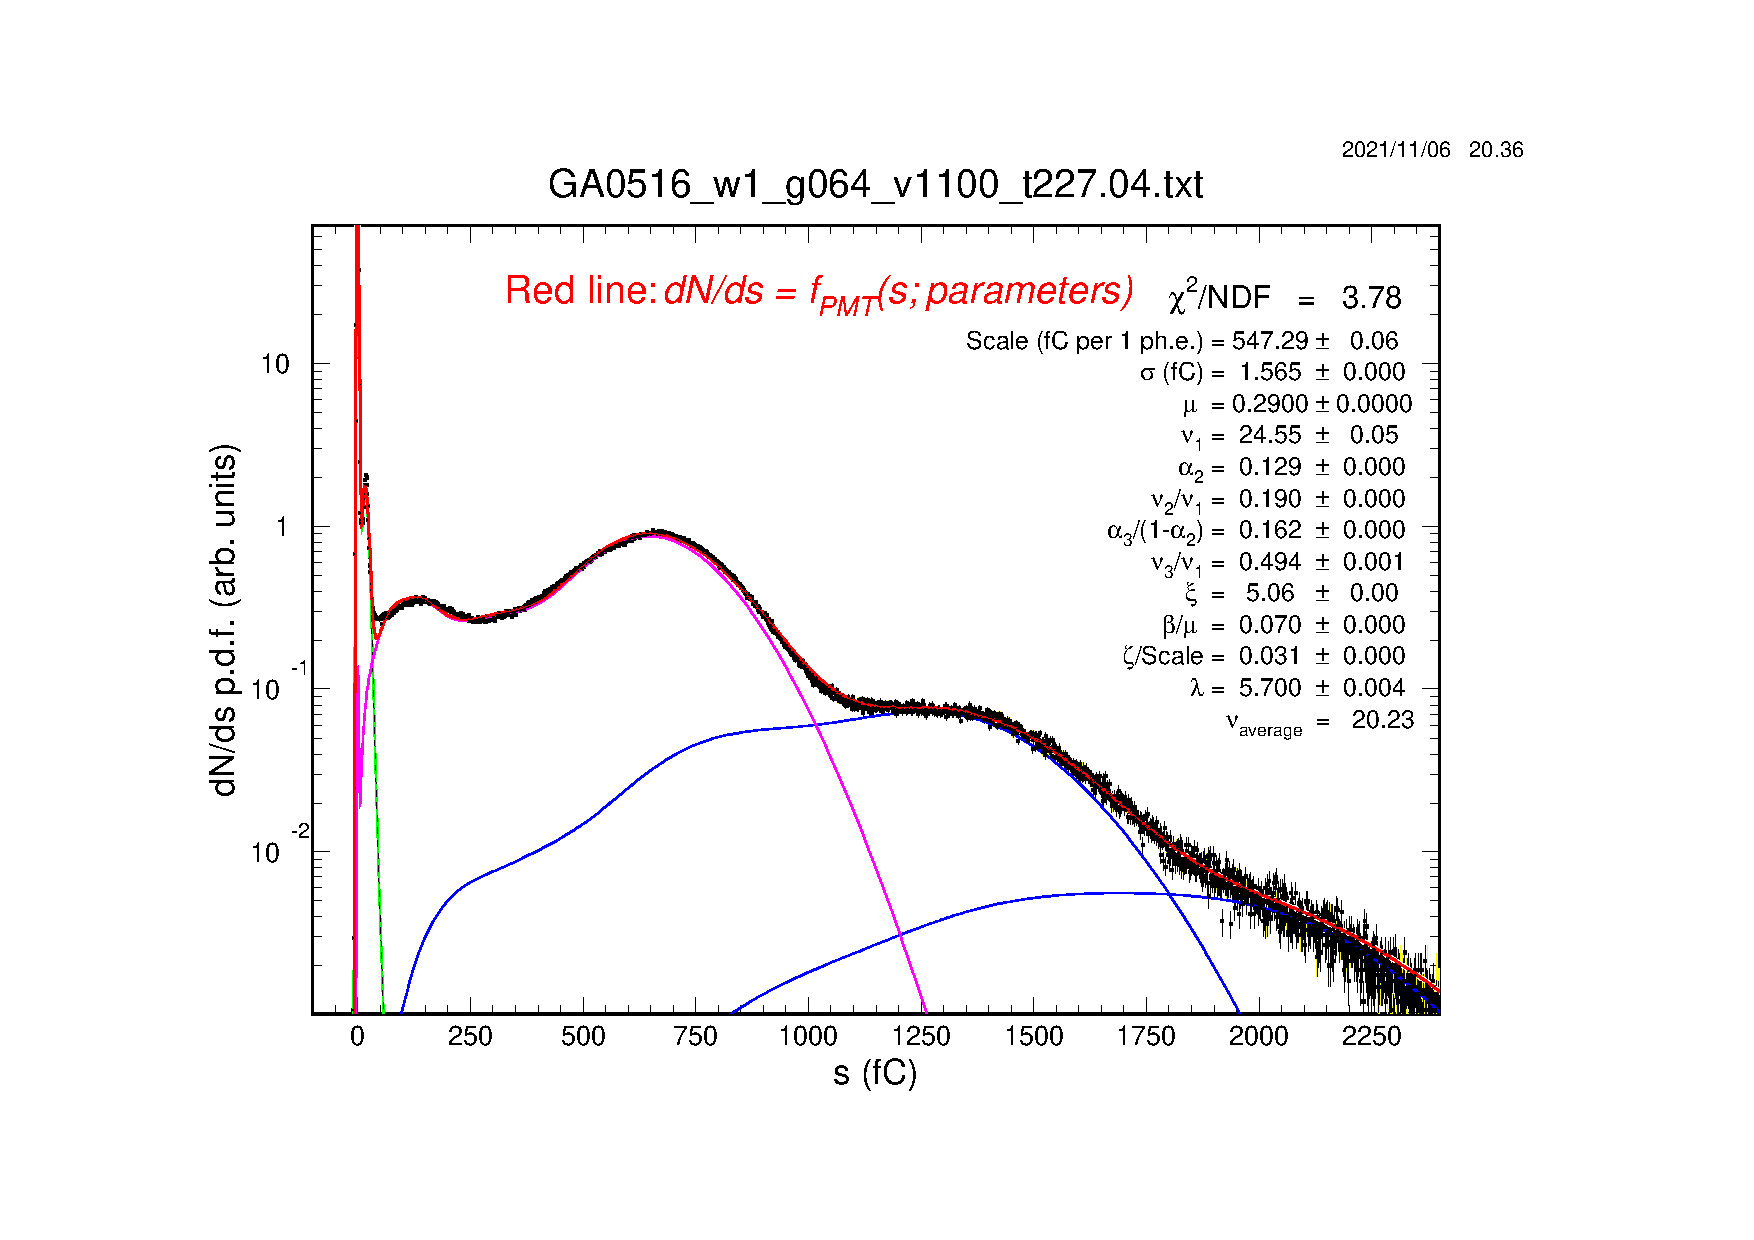
\includegraphics[clip=true,trim=100 75 140 100,width=.245\textwidth,height=.15\textwidth]
                    {figures/GA0516_4b.pdf}}
  \subfloat[No mask, at HV = 1000 V]{%
    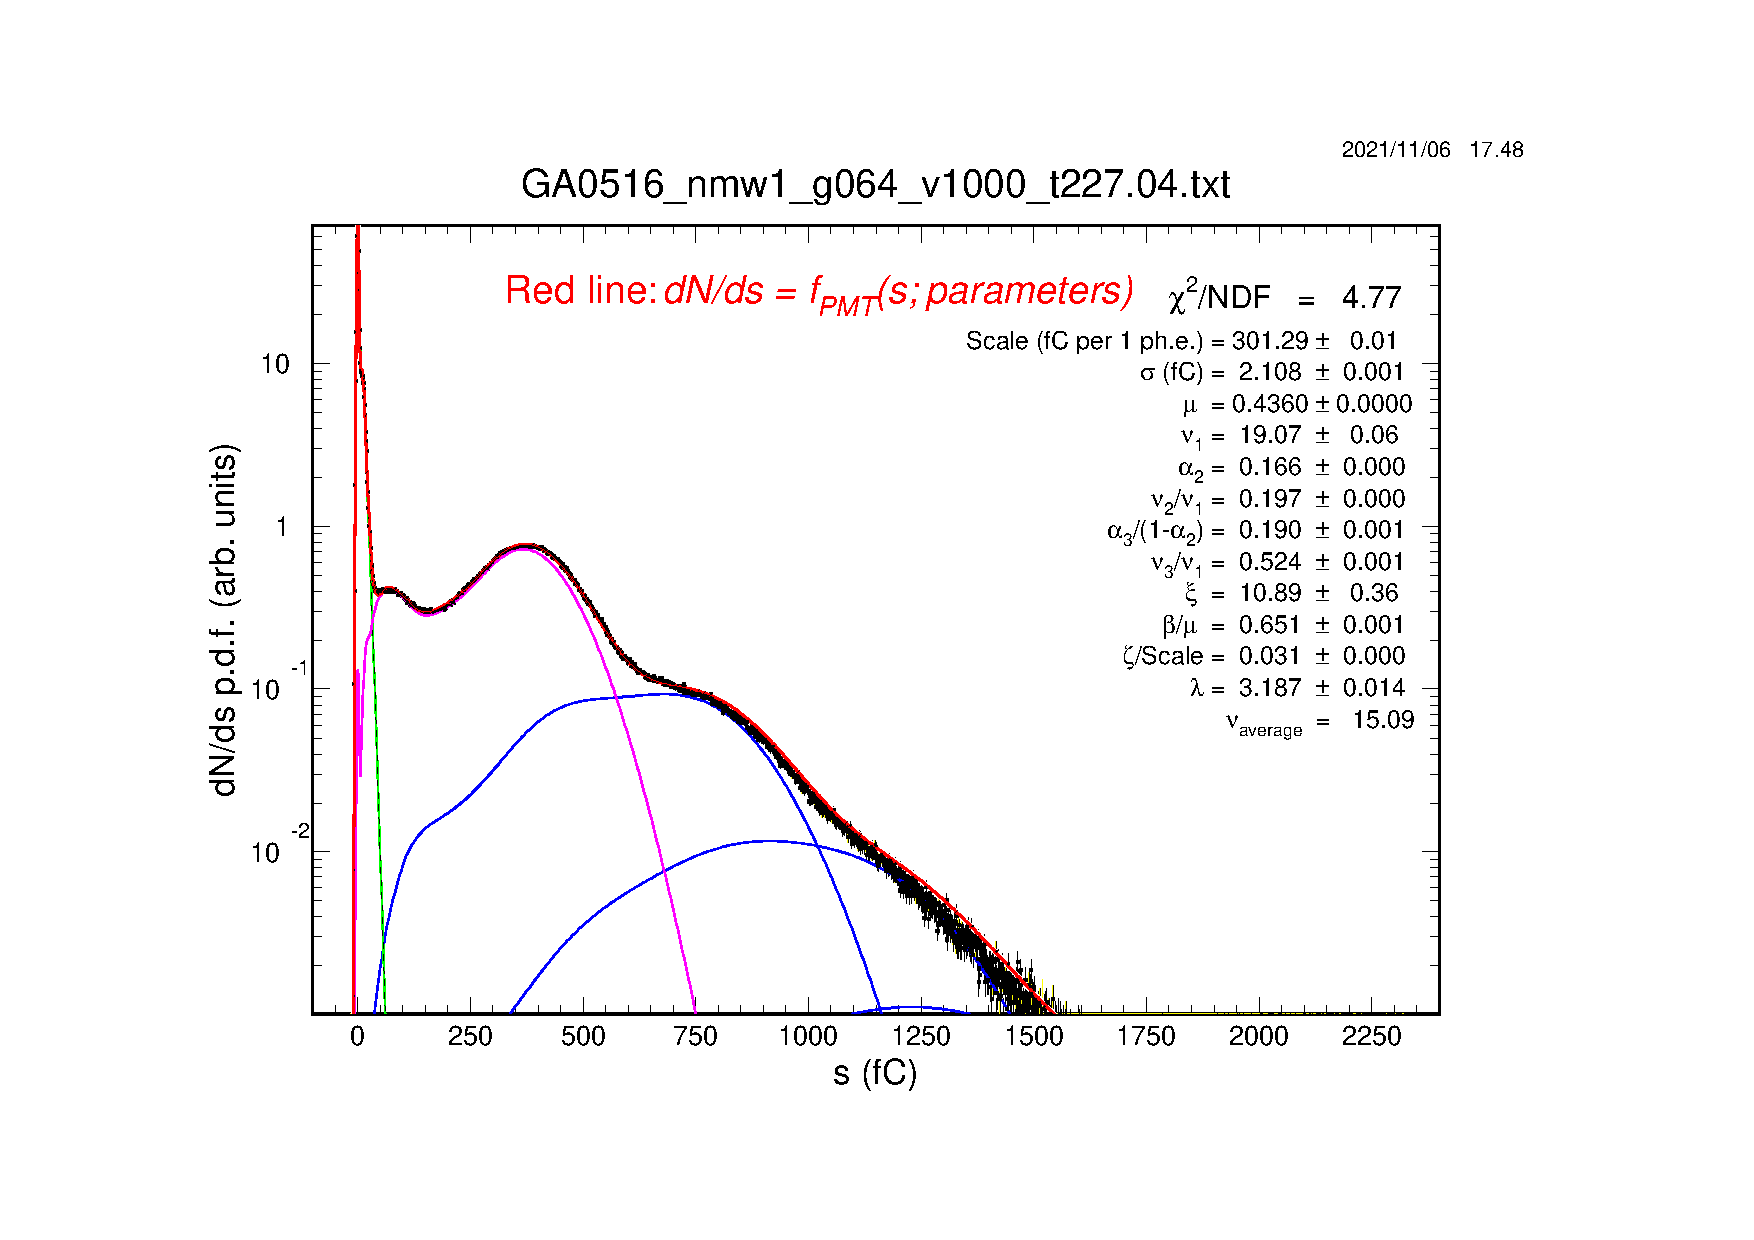
\includegraphics[clip=true,trim=100 75 140 100,width=.245\textwidth,height=.15\textwidth]
                    {figures/GA0516_4c.pdf}}
  \subfloat[No mask, at HV = 1100 V]{%
    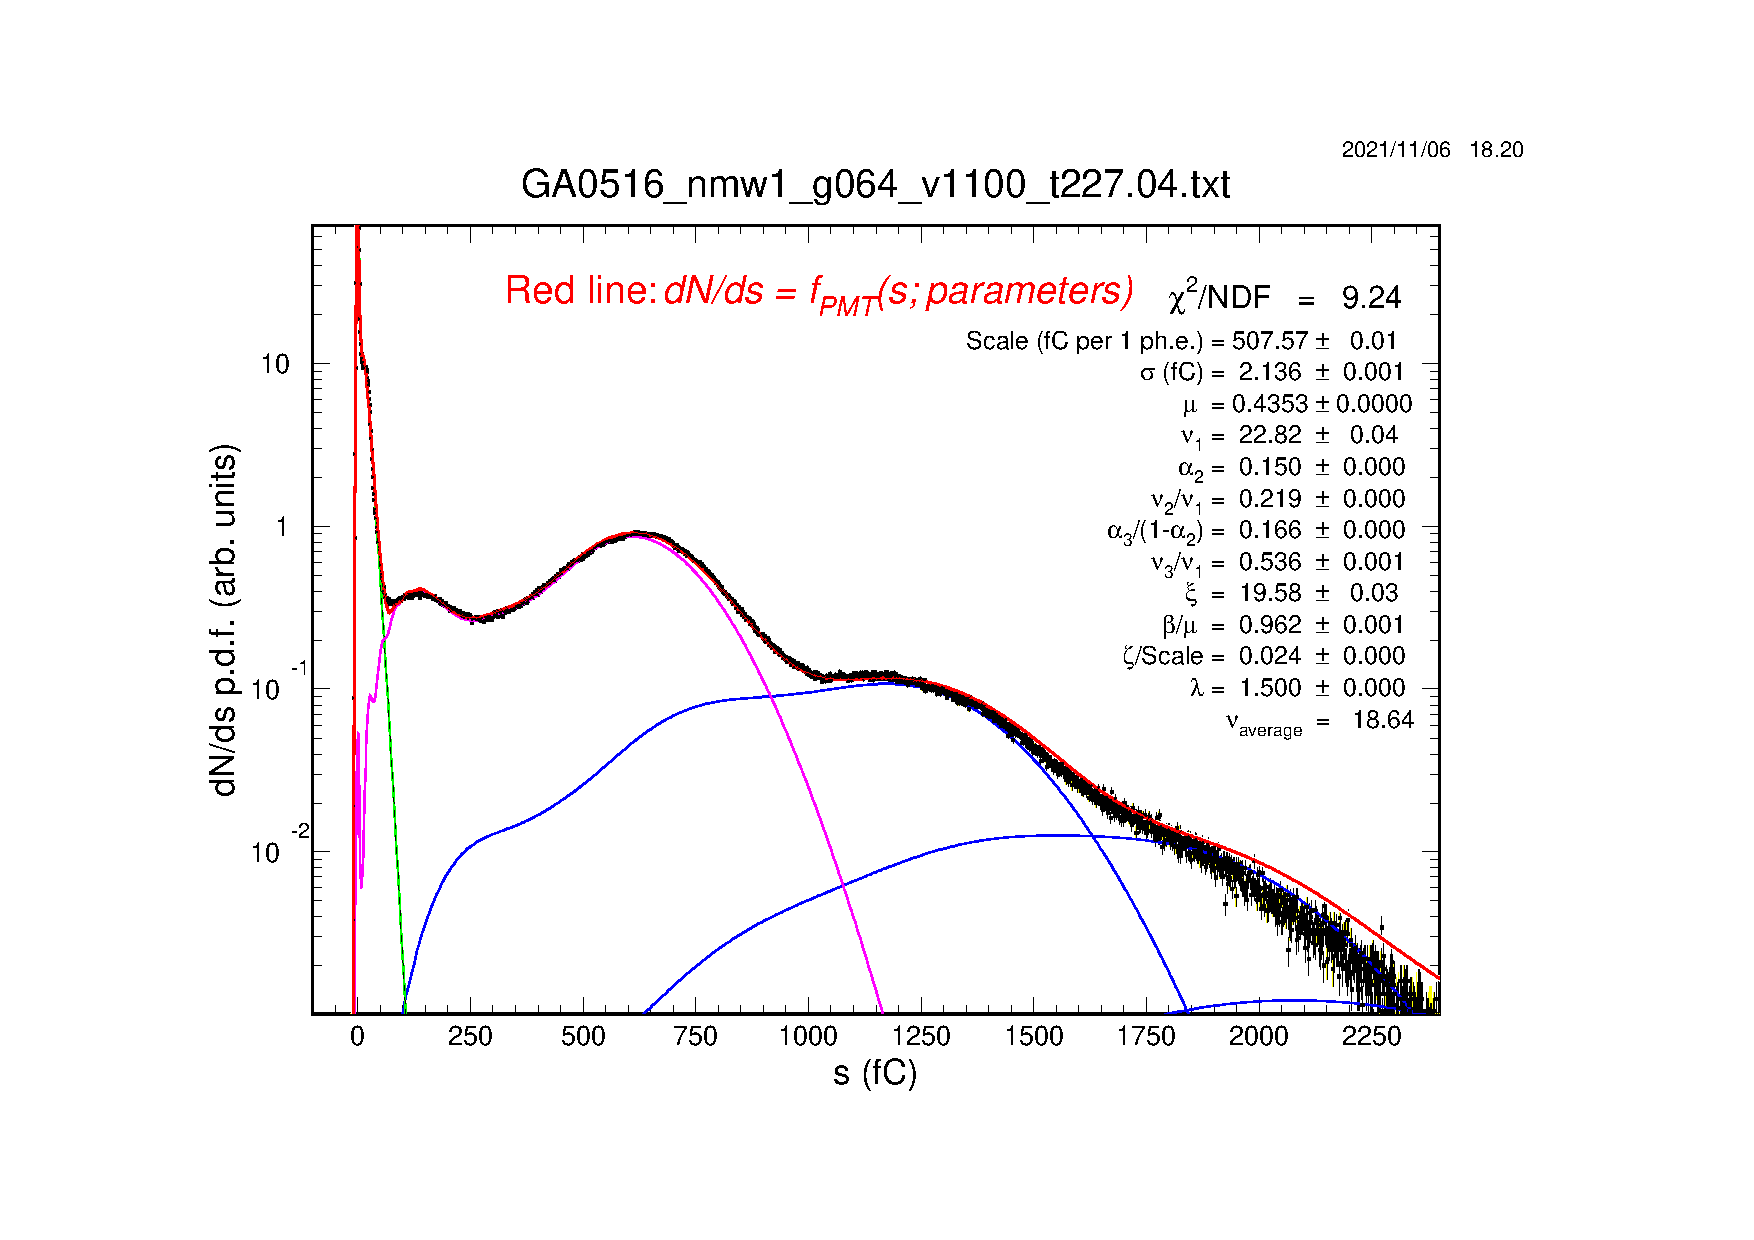
\includegraphics[clip=true,trim=100 75 140 100,width=.245\textwidth,height=.15\textwidth]
                    {figures/GA0516_4d.pdf}}
  \caption{Same as Fig.~\ref{fig:GA0516_3}, but at the wheel position 1. 
    }
\label{fig:GA0516_4}
\end{figure*}


\begin{figure*}[!ht]
	\centering
	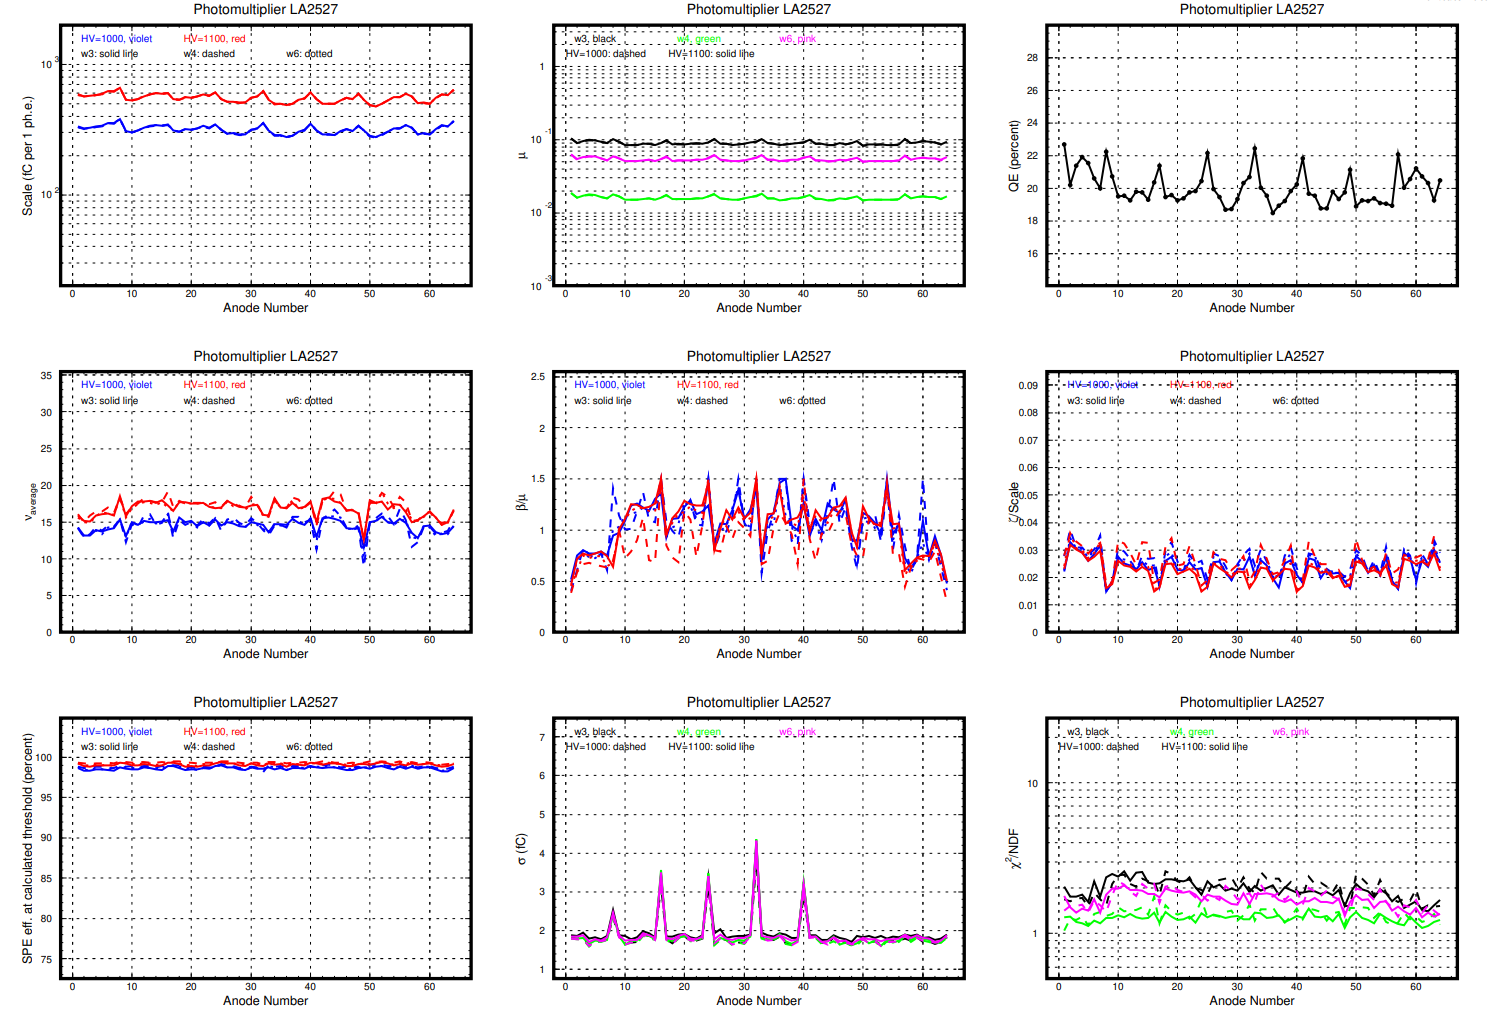
\includegraphics[width=0.9\textwidth,height=.55\textwidth]{figures/pavel_temp/LA2527_passport_temp.png}
	\caption{Illustration of the "MAPMT Passport" plots for one of the tubes, LA2527 (H12700). The standard six measurements included runs at three illumination settings (wheel positions 3, 4, and 6), each at two operating high voltage values (1000 V, and 1100 V).}
	\label{fig:LA2527_passport}
\end{figure*}
\begin{figure*}[!ht]
	\centering
	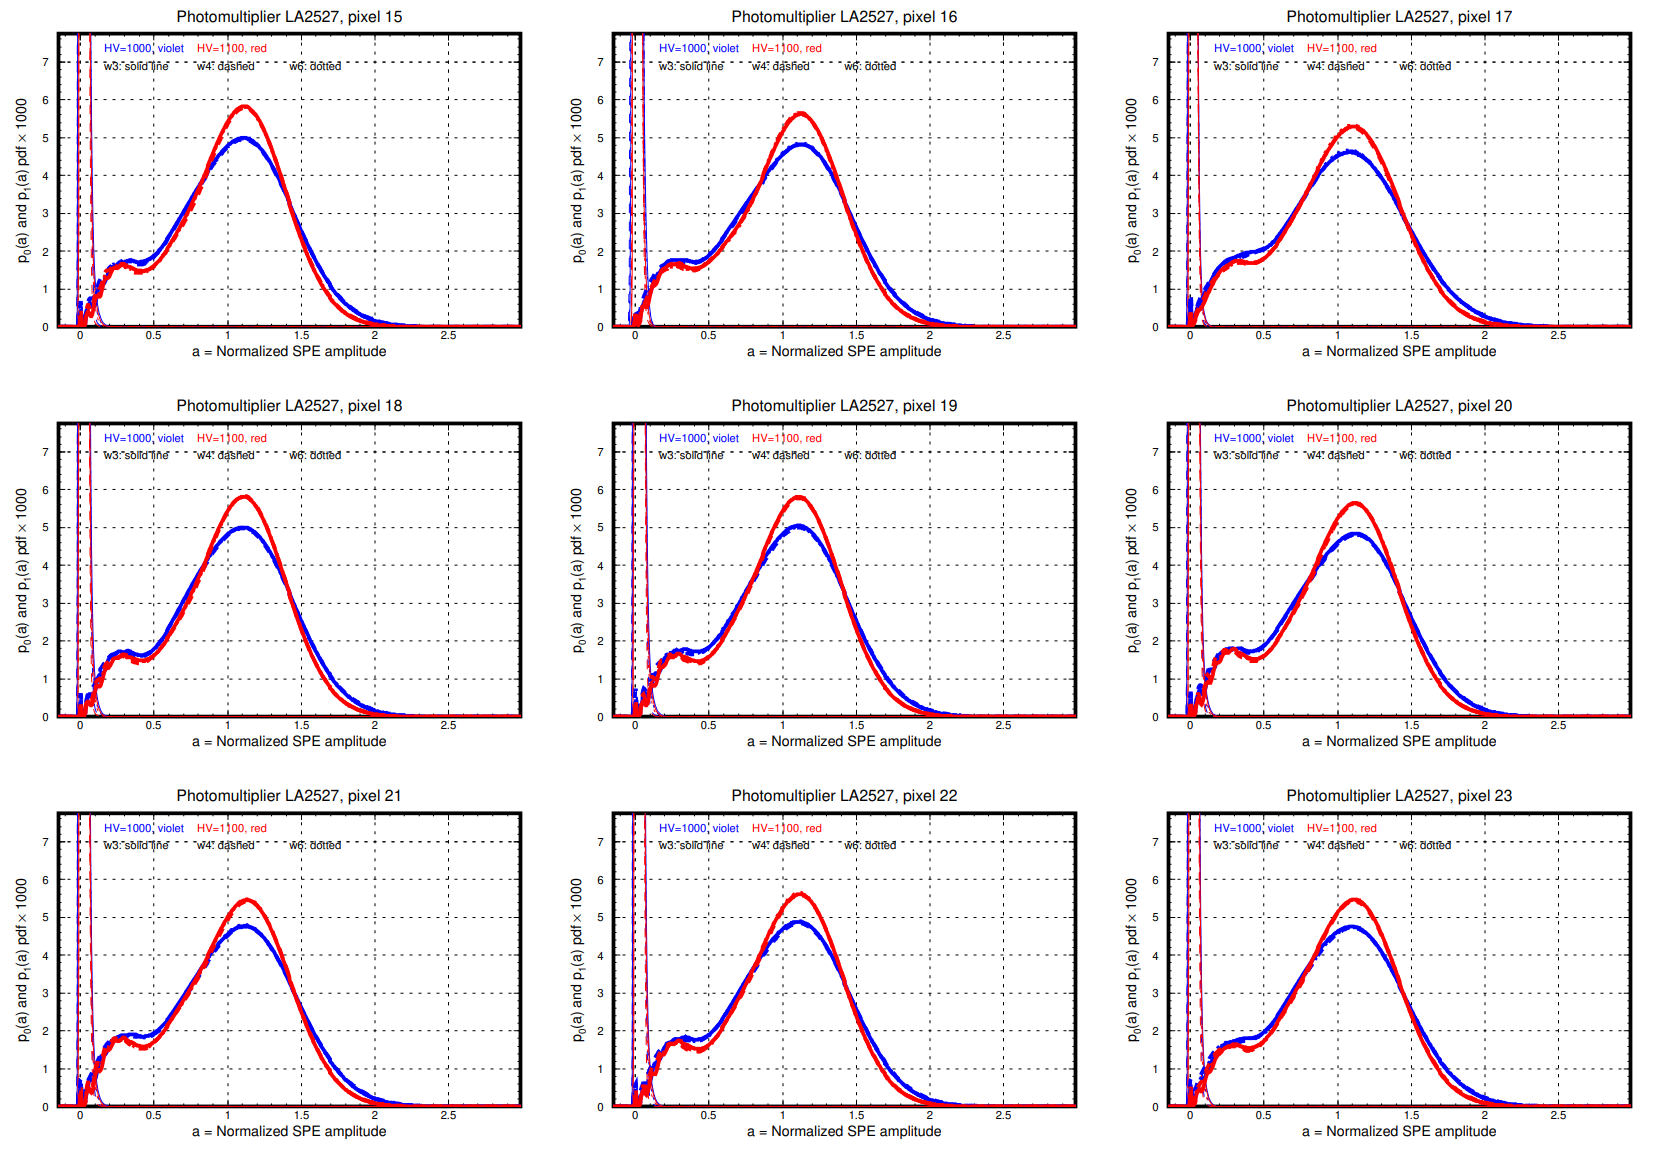
\includegraphics[width=0.9\textwidth,height=.55\textwidth]{figures/pavel_temp/LA2527_spectra_temp.png}
	\caption{Illustration of the "MAPMT Passport" plots for one of the tubes, LA2527 (H12700), continued. The standard six measurements included runs at three illumination settings (wheel positions 3, 4, and 6), each at two operating high voltages (1000 V, and 1100 V). Shown are the calculated SPE functions, defined by the fit parameters resulting from the independent fitting procedures for each six settings. Blue color corresponds to the three sets at HV = 1000 V, and red - to the runs at HV = 1100 V. The fit parameters of the independent fits at three different illuminations result in very stable SPE shapes, essentially overlapping each other in the plots.}
	\label{fig:LA2527_passport_spectra}
\end{figure*}

As a demonstration of the characterization procedure for the MAPMTs, Fig.~\ref{fig:CA7811}-\ref{fig:GA0516_4} show the measured signal amplitude probability distributions for one H8500 MAPMT pixel (CA7811, pixel 9) and one H12700 MAPMT pixel (GA0516, pixel 4) under various conditions, as well as their respective fit results. 
Fig.~\ref{fig:CA7811} and Fig.~\ref{fig:GA0516_1} illustrate the effect that the electronic cross talk from neighboring pixels has on the measured SPE fit parameters. 
We collected two sets of data intended to reduce the contribution of crosstalk from neighboring pixels. 
In the first (as described in Chapter 5) we used a black sheet of paper to mask all pixels on a single MAPMT, and punctured a 3mm hole over the pixel of interest (Fig.~\ref{fig:CA7811}a). 
However, with this setup one cannot fully characterize the unmasked pixel, as there is some dependence of the measured signal on the location of the incident photon. 
To provide full coverage of a single pixel\textquotesingle s surface, another set of measurements was taken with a 6mm x 6mm square hole cut out over a single pixel. 
With this configuration, the full face of the pixel of interest is illuminated, while the neighboring pixels remain mostly covered by the black paper. 
However, there is still non-negligible contribution from crosstalk with this configuration, due to imperfect alignment of the masks. 
This can be clearly seen in Fig.~\ref{fig:CA7811}b which shows the signal amplitude distribution with this 6mm x 6mm square hole cut out over pixel 9. 
One can see the contribution of the crosstalk appearing as a shoulder to the pedestal, albeit smaller than the crosstalk shoulder seen in Fig.~\ref{fig:CA7811}d where the full face of the MAPMT is illuminated. 

The resulting SPE fit parameters for Fig.~\ref{fig:CA7811}a-d indicate the inability of the model to fully describe the crosstalk in the H8500 MAPMTs. 
Most notably, in the data sets where the full-face of the MAPMT was illuminated (Fig.~\ref{fig:CA7811}c and Fig.~\ref{fig:CA7811}d) the $scale$ parameter changes by almost $7\%$ when the crosstalk is removed by the offline correlation analysis procedure compared to when it is kept in the data. 
Because the $scale$ parameter gives the average charge measured per photoelectron, it should be independent of the crosstalk. 
In contrast, we observe that the crosstalk in the H12700 MAPMTs can indeed be well described by the updated model, as is evident by comparing the fit parameters for Fig.~\ref{fig:GA0516_1}c and Fig.~\ref{fig:GA0516_1}d. 
All parameters are consistent between the two fits, despite the fact that the crosstalk was removed by the offline analysis prior to performing the fit for Fig.~\ref{fig:GA0516_1}c. 
This result exemplifies the ability of the model to extract the SPE parameters from the measured signal amplitude distributions in a crosstalk-independent manner. 


The same sets of data were taken with the MAPMT high voltage set to 1100V to compare with the results of Fig.~\ref{fig:GA0516_1} which were taken at 1000V. 
The resulting amplitude probability distributions and fits are shown in Fig.~\ref{fig:GA0516_2}. 
As expected, both the $scale$ and $\nu_{average}$ parameters are larger when the HV is increased to 1100V, while the parameters describing the crosstalk, $\beta/\mu$ and $\zeta/scale$, are fairly consistent. 
Furthermore, by comparing Fig.~\ref{fig:GA0516_2}c and Fig.~\ref{fig:GA0516_2}d, we observe the same desirable characteristic that the SPE fit parameters are consistent with or without the offline removal of the crosstalk events from the data even at a larger high voltage setting.


Finally, Fig.~\ref{fig:GA0516_3} and Fig.~\ref{fig:GA0516_4} show the signal amplitude probability distributions for the same pixel on MAPMT GA0516 at higher illumination intensities. 
Specifically, Fig.~\ref{fig:GA0516_3} shows the results when the filter wheel is at position 2, for HV settings 1000V and 1100V, both with the full MAPMT face illuminated, and with the 6mm x 6mm square hole mask cutout applied. 
Comparing Fig.~\ref{fig:GA0516_3}c to Fig.~\ref{fig:GA0516_1}d (full-face illumination, 1000V), the $\mu$ parameter is almost a factor of 10 larger for the data collected with wheel position 2, but the characteristic parameters for the SPE response are consistent. 
The same can be said by comparing to the signal amplitude probability distribution in Fig.~\ref{fig:GA0516_4}c, which was measured at filter wheel position 1 (highest illumination). 
Even at roughly 100 times the light intensity, the resulting $scale$ parameter is consistent to what is measured at low light intensity. 

Fig.~\ref{fig:LA2527_passport} shows an example of the "Passport" plots obtained for a single MAPMT - in this case, an H12700 PMT labeled LA2527. 
Each plot shows different parameters extracted from the fits to the signal amplitude probability distributions vs. the pixel number, resulting in 64 data points per curve.
In all plots (excluding the top-right plot), the fit results are compared for the data taken with wheel positions 1, 2, and 3, and high voltages 1000V and 1100V (6 different configurations in total).
As expected the $scale$ and $\nu_{average}$ parameters are independent of the light intensity, but change with the applied high voltage. 
This is due to the increased amplification at each dynode at higher applied voltages.
The $\beta/\mu$ and $\zeta/scale$ parameters which describe the PMT crosstalk remain somewhat consistent between the different experimental configurations. 
Moreover, the $\beta/\mu$ passport plot shows the dependence of the crosstalk on pixel location. For example, the first 8 and last 8 pixels all have significantly lower $\beta/\$ is some dependence of the $\beta/\mu$ parameter on the  is consistently lower for the first 8 pixels and for the last 8 pixels than most of the pixels in between.
This is because the first and last 8 pixels are the ones in the top and bottom rows of the MAPMT, meaning there are in general less pixels neighboring them.
Consequently, there is a lower contribution from the crosstalk in these pixels.

One final remark from the plots included in Fig.~\ref{fig:LA2527_passport} is that the SPE efficiency (lower-left plot) is slightly larger at 1100V than at 1000V. The higher voltage leads to increased separation between the SPE spectra and the pedestal, thus increasing the efficiency. 
Fig.~\ref{fig:LA2527_passport_spectra} shows the extracted SPE functions for 9 pixels on the same MAPMT, again for all 6 configurations. The probability distributions are given as a function of the normalized charge amplitude, $a$. The functions extracted from the data measured with 1100V are noticeably more narrow around the peak than the data collected at 1000V.


\iffalse
The performance of MAPMTs was evaluated under certain high voltages.
The single photoelectron spectrum and the pixel efficiency for H12700 MAPMTs were tested and analyzed at 1000v, 1050v, 1075v, and 1100v.
The measurements performed at the reference supply voltage of 1000 V were compared to the measurements at different HV values in order to study the behavior of the MAPMT response as a function of the supply voltage.
As expected, it was found that the H12700 MAPMTs perform the best in the single photoelectron spectrum efficiency at higher voltages, especially at 1100v.
We see a significantly improved separation of the first photoelectron peak from the pedestal at higher voltage supplies (see~Fig.~\ref{fig:SPEhv}).
When the average deficiencies of the tested MAPMTs were analyzed, it was found that the average efficiency for 1000v, 1050v, 1075v and 1100v were approximately 4.6\%, 4.9\%, 5.0\%, and 5.2\%, respectively.
Therefore, the increase in detection efficiency is found to be over 10\% at 1100 V in comparison to 1000 V supply.
This separation is the crucial point for a single photon counting detectors such as CLAS12 RICH, where the occupancy is at the level of one photon per pixel.



It was also found that as the gain of the MAPMT increased, the efficiency ratio of 1100v to 1000v decreased.
The ratio is shown on~Fig.~\ref{fig:effratio} as a function of MAPMT gain reported by Hamamatsu.
The high voltage supply improves the performance of MAPMT dynode system, decreasing the fraction of the single photoelectron events below the pedestal peak.
This indicates that lower gain MAPMTs have a greater difference in the efficiencies at 1100v and 1000v, while higher gain MAPMTs have a smaller difference between the two voltage efficiencies.
The improvement for lower gain MAPMTs is more significant than for higher gain MAPMTs, because the high gain MAPMT has good separation of signal from pedestal even at the reference 1000 V.
Therefore, the low gain MAPMT benefit greatly from higher supply voltage.
The collected data are used to determine what high voltage the MAPMTs should be ran at to acquire the best results when the RICH detector is completed.


The parameters from Pavel's PMT response function are shown on the Fig.~\ref{fig:mu} and \ref{fig:characteristicPars} and correspond to the emission of the photoelectron ($\mu$), its collection and multiplication on the first dynode ($scale$ and $\nu$).
We have omitted other parameters that take into account the resolution effects of readout system or correspond to the cascade multiplication of the secondary electrons as they are out of scope focus of our analysis.
Given our requirements for single photoelectron signal sensitivity MAPMTs of our choice should be able to detect with high probability single photon that reaches photocathode.
In order to achieve this goal MAPMT should have high quantum efficiency of the photocathode as well as high collection efficiency of produced photoelectron combined with substantial signal multiplication to achieve good resolution of SPE peak.
These characteristics were studied in bulk for all 27520 channels (430x64) during the different light conditions and for different supplied HV values.


Fig.~\ref{fig:mu} shows the distribution of parameter $\mu$ which correspond to the average number of the photoelectrons produced during the measurements.
This parameters represents the convolution of the MAPMT photocathode quantum efficiency and laser setup light intensity.
Both characteristics should not depend on HV supply values and it is demonstrated on this figure by comparison of $\mu$ values extracted for the measurements at 1000 V and 1100 V.
However one can change the parameter by varying the laser light intensity which is evident from the left shift of $\mu$ values for lower light intensity measurements.

The other two free parameters are plotted on Fig.~\ref{fig:characteristicPars}.
They correspond to the average number of second-stage electrons produced on the first dynode by photoelectron (see~Fig.~\ref{fig:nu} and average signal amplitude for single photoelectron spectrum (see Fig.~{fig:scale}).
Both parameters characterize mainly the amplifying subsystem of MAPMT and therefore should depend on supplied HV.
The measurements at 1000 V and 1100 V confirm that amplification is improved at higher values of applied high voltage.
Traditionally the second parameter (gain) is often used to describe the amplification abilities of photomultipliers and often used in calibration and reconstruction procedures.
And it was shown that the extracted gains do not depend on the light conditions with a high degree of accuracy.
\fi
